% TEMPLATE for Usenix papers, specifically to meet requirements of
%  USENIX '05
% originally a template for producing IEEE-format articles using LaTeX.
%   written by Matthew Ward, CS Department, Worcester Polytechnic Institute.
% adapted by David Beazley for his excellent SWIG paper in Proceedings,
%   Tcl 96
% turned into a smartass generic template by De Clarke, with thanks to
%   both the above pioneers
% use at your own risk.  Complaints to /dev/null.
% make it two column with no page numbering, default is 10 point

% Munged by Fred Douglis <douglis@research.att.com> 10/97 to separate
% the .sty file from the LaTeX source template, so that people can
% more easily include the .sty file into an existing document.  Also
% changed to more closely follow the style guidelines as represented
% by the Word sample file. 

% Note that since 2010, USENIX does not require endnotes. If you want
% foot of page notes, don't include the endnotes package in the 
% usepackage command, below.

% This version uses the latex2e styles, not the very ancient 2.09 stuff.
\documentclass[letterpaper,twocolumn,10pt]{article}
\usepackage{usenix,epsfig,endnotes}

\usepackage{url}
\usepackage{microtype}
\usepackage{appendix}
\usepackage{epsfig}
\usepackage{amssymb}
\usepackage{amsmath}
\usepackage{amsfonts}
\usepackage{pgfplots}

\begin{document}

%don't want date printed
\date{}

%make title bold and 14 pt font (Latex default is non-bold, 16 pt)
\title{\Large \bf Distinguishing Inputs with the FLUSH+RELOAD Cache Side Channel}

%for single author (just remove % characters)
\author{
{\rm Taylor Hornby}\\
University of Calgary
\and
{\rm John Aycock}\\
University of Calgary
% copy the following lines to add more authors
% \and
% {\rm Name}\\
%Name Institution
} % end author

\maketitle

% Use the following at camera-ready time to suppress page numbers.
% Comment it out when you first submit the paper for review.
\thispagestyle{empty}


\subsection*{Abstract}
Side channel attacks are typically used to break implementations of
cryptography. More recently, side channel attacks have been discovered in more
general settings that violate user privacy. We continue this trend by showing
that the \textsc{Flush+Reload} L3 cache side channel from Yuval Yarom and
Katrina Falkner \cite{yarom2013flush} can be used to distinguish between inputs
to non-cryptographic programs. We do so by presenting three attacks. First, we
attack the Links command-line web browser, showing that an attacker can
determine which of the top 100 Wikipedia pages the user visited (correct 94\% of
the time). Second, we show that an attacker can determine which of a set of 127
PDFs were processed by the poppler PDF rendering library (correct 98\% of the
time). Finally, we show that an attacker can determine whether the TrueCrypt
volume the user just mounted contained a hidden volume or not. We also describe
how to discover new input distinguishing attacks in a partially automated way
(correct above 80\% of the time).

\section{Introduction}
\label{sec:intro}

Side channels are a well-known class of attack where an adversary learns
information about their victim through implicit, rather than explicit,
transmission of information. Transmission of information is accomplished through
media such as radio signals, execution time, power usage, and through the state
of a computer's memory cache.

Side channels are most commonly used to extract secret keys from implementations
of cryptography. For example, Thomas Messerges et al.\ were able to extract the
secret RSA key from a smart card by looking at the amount of power it uses
\cite{messerges1999power}. More recently, Genkin et al.\ were able to extract
a secret RSA key just by listening to the sounds a computer makes as it is
decrypting data \cite{genkin2013rsa}. 

Side channel attacks are also being used to compromise user privacy. For
example, Liang Cai and Hao Chen have shown that keystrokes (including typed PIN
numbers) can be reliably recovered from accelerometer data on smartphones
\cite{cai2012practicality}. Shuo Chen et al.\ showed that observing a web
application's behavior reveals information about the user's input. They gave
real-world examples where they could determine which medical conditions the user
was searching for, what their income range was, and how they allocated their
investment funds \cite{chen2010side}.

In this paper, we continue the trend of using side channels to attack the user's
privacy. We show that the generic L3 cache side channel called
\textsc{Flush+Reload} \cite{yarom2013flush} can be applied in non-cryptography
settings to meaningfully violate confidentiality. We give three examples where
the attack can be used to figure out which of a set of inputs the user gave to
a program. In particular, we show how an attacker on a shared system can (1)
determine which of the top 100 Wikipedia pages the user visited, (2) determine
which of the 127 PDF files the user passed to the \textsc{pdftops} command, and
(3) determine whether the TrueCrypt volume the user just mounted contained
a hidden volume or not.

In addition to the three attacks, we also describe how the process of
discovering new attacks can be partially automated.

To the best of our knowledge, this is the first time that a generic cache-based
side channel has been used to compromise privacy by attacking
a non-cryptographic application. The attacks we present show that cache side
channels have implications beyond just extracting secret keys from cryptography
software. We hope that the attacks will bring more attention to the privacy
issues caused by cache side channels, and the \textsc{Flush+Reload} attack in
particular.

We developed a robust \textsc{Flush+Reload} attack tool based on code the
original paper's authors gave us. Our code is published online under an
open-source license (see Appendix \ref{sec:reproducing}), so other researchers
can quickly reproduce our work and start developing better attacks. The source
code for our experiments and the data they produced is being made available as
well. We hope more researchers will follow our example of making code and data
available at the time of publication.

In the next Section, we summarize the \textsc{Flush+Reload} side channel that
our attacks are based on. Section 3 describes our implementation of the
\textsc{Flush+Reload} attack and explains our experimental methodology. The
attacks and experimental results are given in Section 4. Section 5 describes how
the discovery of new attacks can be partially automated. Section 6 highlights
recent work using side channels to break privacy and explains how our
contributions fit in with that work. Finally we list some ideas for future work
in Section 7, and conclude in Section 8.

\section{The Flush+Reload Attack}

The attacks we present use the \textsc{Flush+Reload} attack by Yuval Yarom and
Katrina Falkner \cite{yarom2013flush}. The side channel was first described by
Bangerter et al.\ \cite{gullasch2011cache} where it was used on AES lookup
tables to extract keys and plaintext during encryption. Yuval Yarom and Katrina
Falkner realized it could be applied more generally to spy on the code a process
executes. It was given the name \textsc{Flush+Reload} and has since been applied
to break GnuPG \cite{yarom2013flush} and OpenSSL \cite{benger2014ooh,
yarom2014recovering}.

Here we give a brief explanation of the \textsc{Flush+Reload} attack with enough
detail to understand our attacks. For all of the details, refer to Yuval Yarom
and Katrina Falkner's paper \cite{yarom2013flush}.

\textsc{Flush+Reload} is a generic L3 (or last-level, in case the system does
not have an L3 cache) cache side channel attack. It takes advantage of
executable code page sharing between processes. If Alice is the first to run
a program, the operating system will load the program into physical memory. When
Bob comes along and runs the same program, instead of loading a second copy into
memory, the operating system will set Bob's page tables to use the copy that was
loaded into memory for Alice. The result is that both Alice and Bob are working
off of the same physical memory. If Bob can determine which cache lines of the
shared memory are present in the cache over time, he can tell which cache lines
Alice's process accesses over time. This is what the \textsc{Flush+Reload}
attack does.

Suppose an attacker knows their victim is running a certain program and would
like to see which code the victim's process is running. \textsc{Flush+Reload}
lets the attacker select a handful of cache lines to watch, called ``probes.''
The attacker flushes those lines out of the cache, waits for a certain number of
clock cycles, then times how long it takes to read those lines. If the read is
fast (i.e. consistent with being in the L3 cache), it means the victim accessed
the line during the waiting period. If the read is slow, the victim did not
access the line. The attacker can repeat the process (flushing, then reloading)
to see which code the victim process is executing over time.

For example, the attack against GnuPG puts probes on the RSA modular
exponentiation routines and uses a waiting time of 2048 clock cycles.
Effectively, the attacker gets a 1.5 MHz resolution view into what the victim's
process is doing \cite{yarom2013flush}.

The attack assumes only one instance of the spied-on program is running at
a time. If multiple instances are running, an access to a probed cache line by
any instance will trigger the probe. Only one attacking process can run at
a time on a CPU core. If a pair of attacking processes have to contend for CPU
time, they will miss measurements. So it is assumed only one attacking process
can run at a time.

In summary, the attacker specifies a few (roughly 1 to 5, where adding more
probes makes the measurements less reliable) probe locations within a binary and
the amount of clock cycles to wait between measurements. As output, the attacker
learns the sequence of probes that were accessed during the waiting periods.

\section{Using \textsc{Flush+Reload} to Distinguish Inputs}

In the previous section we described how an attacker can use
\textsc{Flush+Reload} against a victim process. As output, the attacker gets the
sequence of probes as they were hit over time. In this section, we give a novel
method for distinguishing between a set of possible inputs through the
\textsc{Flush+Reload} side channel. Later, we present actual attacks on Links
and Poppler that use this technique.

In the scenario we are interested in, the attacker knows the victim is going to
run a program on some input. The attacker knows that the input is part of a set
of inputs, all of which are available to the attacker. By spying on the program
with \textsc{Flush+Reload}, the attacker hopes to figure out which input in the
set the program was run on.

For example, suppose Alice has just been diagnosed with an illness, and is using
Wikipedia to research it. The attacker, Mallory, knows Alice was just diagnosed,
and wants to find out which illness she has. Mallory knows that Alice will visit
one of, say, 100 Wikipedia pages that are about illnesses. From the
\textsc{Flush+Reload} output, Mallory is going to try to find out which one.

The first step in the attack is to figure out where to place the
\textsc{Flush+Reload} probes to best distinguish the input. This can be done by
reading the program's code and finding functions whose order of execution are
likely to depend heavily the input. It is possible to do this by hand, but some
automation can make it easier. We describe how to automate it in Section
\textbf{TODO}.

With the probes selected, the attack proceeds in three stages. First, the
attacker goes through a training stage. This must be carried out on the victim's
machine (or a machine sufficiently similar to it)\endnote{It is conceivable that
    the attacker could perform the training phase on a different machine with
similar hardware, but we did not try it.}. Next, the actual attack happens. The
attacker spies on the victim as they execute the program on one of the inputs.
Finally, the attacker uses the training data and output from the attack stage to
recover to determine which input was given to the program.

In the training stage, the attacker simply runs the \textsc{Flush+Reload} attack
tool against themselves as they run the program on every input in the set
multiple times. Each observed probe sequence is saved to a file labeled with the
input that generated it. We refer to the number of times each page is sampled by
$T$. As $T$ increases, the training stage takes longer to perform, but the
accuracy of the attack can increase.

In the attack stage, the attacker runs the \textsc{Flush+Reload} attack tool
against the victim as they pass one of the inputs to the program. The attacker
saves the observed probe sequence to a file.

In the recovery stage, the attacker finds the probe sequence in the training set
that is closest to the one observed from the victim. Closeness, here, is
measured by the Levenshtein distance\cite{levenshtein1966binary}, which is
defined as the smallest number of basic edits (insertions, deletions, and
replacements) needed to bring one string to the other. The attacker computes the
Levenshtein distance between the victim's probe sequence and all of the training
probe sequences, and the one with the smallest Levenshtein distance tells the
attacker which input the victim ran the program on.

Before computing the Levenshtein distance, the probe sequences are first
condensed by collapsing a string of hits to the same probe down into a single
hit of that probe, and then truncated to 1000 characters. An example is shown in
Figure~\ref{figure:probetext}. This is done to make the recovery stage faster,
since the algorithm we use to compute the Levenshtein distance has quadratic
running time.

\begin{figure}
    \centering
\begin{verbatim}
BDBABABABABABABABABABABABCABABCBABCBCABC
ABABABCBABCABCBCBDABABACACADBABDBCBABCBA
BABDBCBABDBCABDBCABDBCABCBCBCBABCBCBABAB
DBABABDABDBCABDABABCABDBCBCBABCBCBABCBCB
ABCABCABDABDCBCABCABCBABDABCABDBCABDBCBA
\end{verbatim}
\caption{The first 200 bytes (of 24,984) of an observed probe sequence while
    visiting the Facebook Wikipedia page in Links. From run links/0015.
    \texttt{A} corresponds to \texttt{kill\_html\_stack\_item()}, \texttt{B} to
    \texttt{html\_stack\_dup()}, \texttt{C} to \texttt{html\_a()}, and
    \texttt{D} to \texttt{parse\_html()}}.
    \label{figure:probetext}
\end{figure}

The training stage can be done either before or after the attack stage, and the
attacker can re-use a training set multiple times, so they only need to train
once to go through with many attacks and recoveries.

\subsection{Using Automation to Find the Best Probes}

The hardest part of discovering a new input distinguishing attack is finding the
set of probes to spy on. We want to find a set of functions whose order of
execution best exhibits the differences between the inputs. One way to do this
is to read the program's code, understand it, and then manually list out some
functions that are heavily involved in processing the input. This takes time and
effort. 

In this section, we present a method for automating probe discovery. We describe
a tool which takes a list of functions as input and produces probe sets that are
good at distinguishing the inputs. The tool requires symbols, but not source
code. So as long as the attacker has access to a non-stripped binary, they can
use the tool to find a good probe set without having a deep understanding of the
program.

The tool first looks at the symbols in the binary to list out all of the
functions. Next, some human intelligence is needed to narrow down the list of
functions into a smaller set that are more likely to depend on the input. This
filtering can be as simple as keeping all functions whose names contain
``\texttt{html}'' to get the list of html-parsing functions, as we have done for
Links, or by looking for functions whose names begin with ``\texttt{Gfx::op}''
to get the list of functions responsible for PDF commands, as we have done for
Poppler.

Once the list of functions has been reduced down to a manageable size (e.g. less
than 100 functions), each potential probe is tested individually. A candidate
probe is tested by placing a GDB breakpoint on the first instruction in the
function and counting the number of times it gets executed as the program is
run. This is done three times for each probe. Twice on one input, giving counts
$c_1$ and $c_2$, and once on a second, different, input, giving the count $c_3$.
A score is given to the probe, equal to $|c_3 - c_1| - |c_2 - c_1|$. This
rewards functions whose counts are stable on the same input but vary on
different inputs, meaning they likely depend on the input. The list of candidate
probes are sorted by their scores, and all but the top dozen are rejected.

The reduced and sorted list of functions is then used to generate all possible
sets of size 4. Sets that contain functions that are within 3 cache lines of
each other are immediately removed. If two probes are two close together, the
CPU may fetch instructions ahead of execution and trigger one whenever another
one is actually executed, in which case there is no point having both probes.
The remaining sets are sorted by the sums of their rank in the input list (which
was sorted by score), and this sorted list is given to the user.

In our attacks, we always used the first probe set in the output list.

The next section describes our implementation of this attack.

\section{Attack Implementation}

The binaries we attacked were built from source. We left symbols in to make it
easier to find the probe locations in the binary. Symbols are not required for
the attack to work, but without them, the discovering the attacks would require
manual reverse engineering work.

The attacks are built on the following tools that we built.

\begin{itemize}
    \item A \textsc{Flush+Reload} attack tool, written in C, takes a binary and probe
        addresses with single-character names as arguments. When probes are hit,
        their single-character names are printed to standard output, with pipe
        characters separating the waiting periods. This tool is
        a re-implementation of the tool the original paper's
        (\cite{yarom2013flush}) authors provided us.

    \item A Ruby class that lets Ruby scripts run the attack tool and monitor
        its output. It provides a callback whenever there is a burst of probe
        hits. This lets the attack script react to events (such as the entire
        execution of a command) without having to continually parse the attack
        tool's output. Our attacks are implemented as Ruby scripts that use this
        class.

    \item A semi-automated attack discovery tool. The tool takes as input a list
        of code addresses in the program and two different inputs to the
        program. It produces a list of probe sets that are likely able to
        distinguish between the two inputs. We describe how this tool is used in
        Section 5.

    \item A Ruby implementation of the attack procedure described in Section
          \textbf{TODO}.
\end{itemize}

Before getting into the attacks, we describe our experimental setup in the next
section.

\section{Experiment Setup}

We ran experiments on two systems. The first system is a laptop; the second
system is a dedicated server hosting a low-traffic website and operating as
a relay for the Tor network. The specifications of these systems are given in
Table \ref{table:specs}. We will refer to these systems as System 1 and System
2, respectively.

\begin{table*}
    \centering
\begin{tabular}{|c|c|c|}
    \hline
    & \textbf{System 1} & \textbf{System 2} \\
    \hline
    \textbf{Use} & Laptop & Web server \\
    \hline
    \textbf{OS} & Arch Linux (February 2015) & Debian Wheezy \\
    \hline
    \textbf{CPU} & Intel Core2 Duo P8700 2.53GHz & Intel Xeon E3-1245 V2 3.40GHz  \\
    \hline
    \textbf{RAM} & 4GiB DDR2 800MHz & 32GiB DDR3 1333MHz \\
    \hline
    \textbf{L1 Cache} & 64KiB Split & 256KiB Unified \\
    \hline
    \textbf{L2 Cache} & 3MiB Unified & 1MiB Unified \\
    \hline
    \textbf{L3 Cache} & None & 8MiB Unified \\
    \hline
\end{tabular}
\caption{System specifications. Cache specifications were obtained by the
\texttt{dmidecode} utility and may not be accurate. System 1 does not have a L3
cache, but FLUSH+RELOAD works with its L2 cache as it is shared between cores.}
\label{table:specs}
\end{table*}

To test the input distinguishing attacks, the experiments first perform the
training stage, taking $T$ samples of each input. Then, for every input in the
set of size $N$, the vulnerable program is run on the input $S$ times. The probe
sequences from each of the $SN$ runs are put through the recovery stage
independently, and we check how many of the recoveries were correct.

All of the experiments have been automated so that they are easy to repeat. The
source code and data from all experiment runs have been published so that other
researchers can verify and reproduce our work, see Appendix
\ref{sec:reproducing}.

All experiments were run with low system load.

To make sure that we did not cherry pick vulnerable programs, we kept track of
all the programs we looked at without developing any attacks. These are
disclosed in Section \ref{sec:failures}.

\section{Attacks}
\label{sec:results}

We present three attacks. The first attack lets an attacker tell whether which
of the top 100 Wikipedia pages the victim visited using the Links web browser.
The second attack does the same for the Poppler PDF rendering library,
distinguishing between 127 PDF transcripts of 2014 Canadian parliamentary
debates. The Links and Poppler attacks both use the input distinguishing process
described above. The third attack, which is implemented differently, determines
whether a mounted TrueCrypt volume contained a hidden volume or not.

For the Links and Poppler attacks, we give the probe locations and report the
success rate that we saw in our experiments. For the TrueCrypt attack, we
describe how it works and report the success rate.

\subsection{Links}

Links is a command-line web browser. We are interested in learning which web
page a user is visiting, out of a set of known pages. We found that it is
possible to reliably distinguish between the top 100 Wikipedia pages of
2013~\cite{wikitop2013}.

To find the Links probes, we ran the automated probe finding tool on the HTML
parsing functions inside links. The names of these functions all contain the
string ``html'', so we grepped the list of all functions for ``html'' and gave
the resulting list of 77 functions to the probe finding tool. The two inputs we
gave to the probe finding tool were, for no particular reason, the ``Bird'' and
``Feather'' Wikipedia pages. The tool gave us the following probe set:

\begin{itemize}
    \item \texttt{html\_stack\_item()}
    \item \texttt{html\_stack\_dup()}
    \item \texttt{html\_a()}
    \item \texttt{parse\_html()}
\end{itemize}

On System 1 with $T=10$ and $S=10$ \endnote{links/0014}, the correct page was
identified $940$ times out of $1000$, an accuracy of 94\%. In this experiment,
the average time it took to recover the name of the page from the training
sequences and the victim sequence was $4.1$ seconds. All pages in the set were
correctly identified at least twice out of the ten runs. Most were correctly
identified all 10 times. The distribution is plotted in
Figure~\ref{figure:distribution}.


\begin{figure}
    \centering
    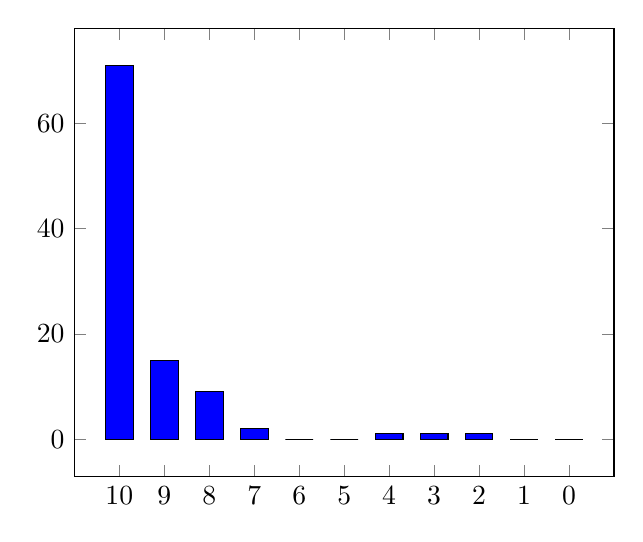
\begin{tikzpicture}
        \begin{axis}[
            symbolic x coords={10, 9, 8, 7, 6, 5, 4, 3, 2, 1, 0},
            xtick=data
          ]
            \addplot[ybar,fill=blue] coordinates {
                (10,   71)
                (9,   15)
                (8,   9)
                (7,   2)
                (6,   0)
                (5,   0)
                (4,   1)
                (3,   1)
                (2,   1)
                (1,   0)
                (0,   0)
            };
        \end{axis}
    \end{tikzpicture}
    \caption{The distribution of success rates for individual pages. On the $x$
        axis, the number of times the page was correctly identified out of ten
        trials. On the $y$ axis, the number of pages that were correctly
        identified that many times. Most pages were correctly identified in all
        ten trials.}
    \label{figure:distribution}
\end{figure}

A second run on System 1 with $T=10$ and $S=1$\endnote{links/0013} saw the
correct page being identified $95$ times out of $100$, an accuracy of 95\%.
Here, it again took $4.1$ seconds to perform a recovery, on average.

On System 2 with $T=10$ and $S=1$\endnote{links/0015}, the correct page was
identified $98$ times out of $100$. Recovery took $136$ seconds on average.
Recovery took much longer on System 2, even though it has better hardware,
because at the time this experiment was run, System 2 was configured to use
a pure Ruby implementation of the Levenshtein distance instead of the fast
native implementation that System 1 was using.

A plot of the Levenshtein distances involved in a successful recovery is shown
in Figure~\ref{figure:youtube}, and an unsuccessful recovery in
Figure~\ref{figure:minaj}.

All of the Wikipedia pages in the set have distinct lengths. So, it is
reasonable to ask whether this attack is just distinguishing the pages by their
lengths. We know this is not the case, however, because the probe sequences are
truncated to 1000 characters before the Levenshtein distance is computed, and in
all of the experiment runs mentioned above, most of the training samples have
lengths above 1000 and so most of the comparisons are between constant-length
strings. So the order of the probe hits matters, and therefore we are really
learning information about the content of the page, and not just its length.

Before we built the probe finding tool, we ran experiments with a different set
of probes that we found manually. We chose these probes by trial and error, and
by looking through the Links source code to find functions whose order of
execution should depend on the contents of Wikipedia pages. These are:

\begin{itemize}
    \item \texttt{parse\_html()}
    \item \texttt{html\_stack\_dup()}
    \item \texttt{html\_h()}
    \item \texttt{html\_span()}
\end{itemize}

With these probes, we saw 76\% accuracy on System 1 with $T=5$ and
$S=1$\endnote{links/0002. This experiment was run before we started truncating
to 1000 characters, so the full strings were compared.}. On System 2 with $T=5$
and $S=10$\endnote{links/0010} we saw 88\% accuracy. With $T=10$ and
$S=1$\endnote{links/0005. This experiment was also run before we started
truncating to 1000 characters.} we saw 91\% accuracy. This indicates that using
more training samples increases the accuracy of the attack, and that the
automatically discovered probes are just as good or slightly better than the
ones we found manually.

\begin{figure*}
    \centering
    % GNUPLOT: LaTeX picture
\setlength{\unitlength}{0.240900pt}
\ifx\plotpoint\undefined\newsavebox{\plotpoint}\fi
\sbox{\plotpoint}{\rule[-0.200pt]{0.400pt}{0.400pt}}%
\begin{picture}(1500,900)(0,0)
\sbox{\plotpoint}{\rule[-0.200pt]{0.400pt}{0.400pt}}%
\put(171.0,131.0){\rule[-0.200pt]{4.818pt}{0.400pt}}
\put(151,131){\makebox(0,0)[r]{ 0}}
\put(1419.0,131.0){\rule[-0.200pt]{4.818pt}{0.400pt}}
\put(171.0,222.0){\rule[-0.200pt]{4.818pt}{0.400pt}}
\put(151,222){\makebox(0,0)[r]{ 100}}
\put(1419.0,222.0){\rule[-0.200pt]{4.818pt}{0.400pt}}
\put(171.0,313.0){\rule[-0.200pt]{4.818pt}{0.400pt}}
\put(151,313){\makebox(0,0)[r]{ 200}}
\put(1419.0,313.0){\rule[-0.200pt]{4.818pt}{0.400pt}}
\put(171.0,404.0){\rule[-0.200pt]{4.818pt}{0.400pt}}
\put(151,404){\makebox(0,0)[r]{ 300}}
\put(1419.0,404.0){\rule[-0.200pt]{4.818pt}{0.400pt}}
\put(171.0,495.0){\rule[-0.200pt]{4.818pt}{0.400pt}}
\put(151,495){\makebox(0,0)[r]{ 400}}
\put(1419.0,495.0){\rule[-0.200pt]{4.818pt}{0.400pt}}
\put(171.0,586.0){\rule[-0.200pt]{4.818pt}{0.400pt}}
\put(151,586){\makebox(0,0)[r]{ 500}}
\put(1419.0,586.0){\rule[-0.200pt]{4.818pt}{0.400pt}}
\put(171.0,677.0){\rule[-0.200pt]{4.818pt}{0.400pt}}
\put(151,677){\makebox(0,0)[r]{ 600}}
\put(1419.0,677.0){\rule[-0.200pt]{4.818pt}{0.400pt}}
\put(171.0,768.0){\rule[-0.200pt]{4.818pt}{0.400pt}}
\put(151,768){\makebox(0,0)[r]{ 700}}
\put(1419.0,768.0){\rule[-0.200pt]{4.818pt}{0.400pt}}
\put(171.0,859.0){\rule[-0.200pt]{4.818pt}{0.400pt}}
\put(151,859){\makebox(0,0)[r]{ 800}}
\put(1419.0,859.0){\rule[-0.200pt]{4.818pt}{0.400pt}}
\put(171.0,131.0){\rule[-0.200pt]{0.400pt}{4.818pt}}
\put(171,90){\makebox(0,0){ 0}}
\put(171.0,839.0){\rule[-0.200pt]{0.400pt}{4.818pt}}
\put(298.0,131.0){\rule[-0.200pt]{0.400pt}{4.818pt}}
\put(298,90){\makebox(0,0){ 10}}
\put(298.0,839.0){\rule[-0.200pt]{0.400pt}{4.818pt}}
\put(425.0,131.0){\rule[-0.200pt]{0.400pt}{4.818pt}}
\put(425,90){\makebox(0,0){ 20}}
\put(425.0,839.0){\rule[-0.200pt]{0.400pt}{4.818pt}}
\put(551.0,131.0){\rule[-0.200pt]{0.400pt}{4.818pt}}
\put(551,90){\makebox(0,0){ 30}}
\put(551.0,839.0){\rule[-0.200pt]{0.400pt}{4.818pt}}
\put(678.0,131.0){\rule[-0.200pt]{0.400pt}{4.818pt}}
\put(678,90){\makebox(0,0){ 40}}
\put(678.0,839.0){\rule[-0.200pt]{0.400pt}{4.818pt}}
\put(805.0,131.0){\rule[-0.200pt]{0.400pt}{4.818pt}}
\put(805,90){\makebox(0,0){ 50}}
\put(805.0,839.0){\rule[-0.200pt]{0.400pt}{4.818pt}}
\put(932.0,131.0){\rule[-0.200pt]{0.400pt}{4.818pt}}
\put(932,90){\makebox(0,0){ 60}}
\put(932.0,839.0){\rule[-0.200pt]{0.400pt}{4.818pt}}
\put(1059.0,131.0){\rule[-0.200pt]{0.400pt}{4.818pt}}
\put(1059,90){\makebox(0,0){ 70}}
\put(1059.0,839.0){\rule[-0.200pt]{0.400pt}{4.818pt}}
\put(1185.0,131.0){\rule[-0.200pt]{0.400pt}{4.818pt}}
\put(1185,90){\makebox(0,0){ 80}}
\put(1185.0,839.0){\rule[-0.200pt]{0.400pt}{4.818pt}}
\put(1312.0,131.0){\rule[-0.200pt]{0.400pt}{4.818pt}}
\put(1312,90){\makebox(0,0){ 90}}
\put(1312.0,839.0){\rule[-0.200pt]{0.400pt}{4.818pt}}
\put(1439.0,131.0){\rule[-0.200pt]{0.400pt}{4.818pt}}
\put(1439,90){\makebox(0,0){ 100}}
\put(1439.0,839.0){\rule[-0.200pt]{0.400pt}{4.818pt}}
\put(171.0,131.0){\rule[-0.200pt]{0.400pt}{175.375pt}}
\put(171.0,131.0){\rule[-0.200pt]{305.461pt}{0.400pt}}
\put(30,495){\makebox(0,0){\rotatebox{90}{Levenshtein Distance}}}
\put(805,29){\makebox(0,0){Page}}
\put(171,338){\makebox(0,0){$+$}}
\put(184,359){\makebox(0,0){$+$}}
\put(196,400){\makebox(0,0){$+$}}
\put(209,412){\makebox(0,0){$+$}}
\put(222,385){\makebox(0,0){$+$}}
\put(234,380){\makebox(0,0){$+$}}
\put(247,432){\makebox(0,0){$+$}}
\put(260,483){\makebox(0,0){$+$}}
\put(272,434){\makebox(0,0){$+$}}
\put(285,341){\makebox(0,0){$+$}}
\put(298,431){\makebox(0,0){$+$}}
\put(310,425){\makebox(0,0){$+$}}
\put(323,365){\makebox(0,0){$+$}}
\put(336,417){\makebox(0,0){$+$}}
\put(349,361){\makebox(0,0){$+$}}
\put(361,393){\makebox(0,0){$+$}}
\put(374,450){\makebox(0,0){$+$}}
\put(387,402){\makebox(0,0){$+$}}
\put(399,345){\makebox(0,0){$+$}}
\put(412,380){\makebox(0,0){$+$}}
\put(425,400){\makebox(0,0){$+$}}
\put(437,409){\makebox(0,0){$+$}}
\put(450,439){\makebox(0,0){$+$}}
\put(463,453){\makebox(0,0){$+$}}
\put(475,353){\makebox(0,0){$+$}}
\put(488,405){\makebox(0,0){$+$}}
\put(501,480){\makebox(0,0){$+$}}
\put(513,371){\makebox(0,0){$+$}}
\put(526,783){\makebox(0,0){$+$}}
\put(539,424){\makebox(0,0){$+$}}
\put(551,409){\makebox(0,0){$+$}}
\put(564,396){\makebox(0,0){$+$}}
\put(577,429){\makebox(0,0){$+$}}
\put(589,351){\makebox(0,0){$+$}}
\put(602,391){\makebox(0,0){$+$}}
\put(615,417){\makebox(0,0){$+$}}
\put(627,346){\makebox(0,0){$+$}}
\put(640,471){\makebox(0,0){$+$}}
\put(653,452){\makebox(0,0){$+$}}
\put(666,350){\makebox(0,0){$+$}}
\put(678,434){\makebox(0,0){$+$}}
\put(691,360){\makebox(0,0){$+$}}
\put(704,359){\makebox(0,0){$+$}}
\put(716,402){\makebox(0,0){$+$}}
\put(729,361){\makebox(0,0){$+$}}
\put(742,403){\makebox(0,0){$+$}}
\put(754,471){\makebox(0,0){$+$}}
\put(767,371){\makebox(0,0){$+$}}
\put(780,349){\makebox(0,0){$+$}}
\put(792,460){\makebox(0,0){$+$}}
\put(805,356){\makebox(0,0){$+$}}
\put(818,439){\makebox(0,0){$+$}}
\put(830,466){\makebox(0,0){$+$}}
\put(843,462){\makebox(0,0){$+$}}
\put(856,444){\makebox(0,0){$+$}}
\put(868,389){\makebox(0,0){$+$}}
\put(881,420){\makebox(0,0){$+$}}
\put(894,450){\makebox(0,0){$+$}}
\put(906,387){\makebox(0,0){$+$}}
\put(919,565){\makebox(0,0){$+$}}
\put(932,419){\makebox(0,0){$+$}}
\put(944,392){\makebox(0,0){$+$}}
\put(957,376){\makebox(0,0){$+$}}
\put(970,420){\makebox(0,0){$+$}}
\put(983,392){\makebox(0,0){$+$}}
\put(995,346){\makebox(0,0){$+$}}
\put(1008,375){\makebox(0,0){$+$}}
\put(1021,285){\makebox(0,0){$+$}}
\put(1033,440){\makebox(0,0){$+$}}
\put(1046,404){\makebox(0,0){$+$}}
\put(1059,367){\makebox(0,0){$+$}}
\put(1071,409){\makebox(0,0){$+$}}
\put(1084,411){\makebox(0,0){$+$}}
\put(1097,381){\makebox(0,0){$+$}}
\put(1109,424){\makebox(0,0){$+$}}
\put(1122,376){\makebox(0,0){$+$}}
\put(1135,361){\makebox(0,0){$+$}}
\put(1147,329){\makebox(0,0){$+$}}
\put(1160,505){\makebox(0,0){$+$}}
\put(1173,343){\makebox(0,0){$+$}}
\put(1185,348){\makebox(0,0){$+$}}
\put(1198,416){\makebox(0,0){$+$}}
\put(1211,410){\makebox(0,0){$+$}}
\put(1223,388){\makebox(0,0){$+$}}
\put(1236,347){\makebox(0,0){$+$}}
\put(1249,371){\makebox(0,0){$+$}}
\put(1261,414){\makebox(0,0){$+$}}
\put(1274,499){\makebox(0,0){$+$}}
\put(1287,402){\makebox(0,0){$+$}}
\put(1300,426){\makebox(0,0){$+$}}
\put(1312,370){\makebox(0,0){$+$}}
\put(1325,403){\makebox(0,0){$+$}}
\put(1338,530){\makebox(0,0){$+$}}
\put(1350,437){\makebox(0,0){$+$}}
\put(1363,357){\makebox(0,0){$+$}}
\put(1376,342){\makebox(0,0){$+$}}
\put(1388,427){\makebox(0,0){$+$}}
\put(1401,382){\makebox(0,0){$+$}}
\put(1414,447){\makebox(0,0){$+$}}
\put(1426,346){\makebox(0,0){$+$}}
\put(171,406){\makebox(0,0){$\times$}}
\put(184,362){\makebox(0,0){$\times$}}
\put(196,410){\makebox(0,0){$\times$}}
\put(209,409){\makebox(0,0){$\times$}}
\put(222,409){\makebox(0,0){$\times$}}
\put(234,399){\makebox(0,0){$\times$}}
\put(247,458){\makebox(0,0){$\times$}}
\put(260,487){\makebox(0,0){$\times$}}
\put(272,418){\makebox(0,0){$\times$}}
\put(285,343){\makebox(0,0){$\times$}}
\put(298,428){\makebox(0,0){$\times$}}
\put(310,421){\makebox(0,0){$\times$}}
\put(323,368){\makebox(0,0){$\times$}}
\put(336,423){\makebox(0,0){$\times$}}
\put(349,377){\makebox(0,0){$\times$}}
\put(361,356){\makebox(0,0){$\times$}}
\put(374,441){\makebox(0,0){$\times$}}
\put(387,405){\makebox(0,0){$\times$}}
\put(399,345){\makebox(0,0){$\times$}}
\put(412,428){\makebox(0,0){$\times$}}
\put(425,375){\makebox(0,0){$\times$}}
\put(437,418){\makebox(0,0){$\times$}}
\put(450,430){\makebox(0,0){$\times$}}
\put(463,446){\makebox(0,0){$\times$}}
\put(475,372){\makebox(0,0){$\times$}}
\put(488,402){\makebox(0,0){$\times$}}
\put(501,473){\makebox(0,0){$\times$}}
\put(513,415){\makebox(0,0){$\times$}}
\put(526,781){\makebox(0,0){$\times$}}
\put(539,434){\makebox(0,0){$\times$}}
\put(551,388){\makebox(0,0){$\times$}}
\put(564,396){\makebox(0,0){$\times$}}
\put(577,398){\makebox(0,0){$\times$}}
\put(589,330){\makebox(0,0){$\times$}}
\put(602,385){\makebox(0,0){$\times$}}
\put(615,411){\makebox(0,0){$\times$}}
\put(627,356){\makebox(0,0){$\times$}}
\put(640,477){\makebox(0,0){$\times$}}
\put(653,457){\makebox(0,0){$\times$}}
\put(666,343){\makebox(0,0){$\times$}}
\put(678,388){\makebox(0,0){$\times$}}
\put(691,376){\makebox(0,0){$\times$}}
\put(704,368){\makebox(0,0){$\times$}}
\put(716,409){\makebox(0,0){$\times$}}
\put(729,366){\makebox(0,0){$\times$}}
\put(742,405){\makebox(0,0){$\times$}}
\put(754,465){\makebox(0,0){$\times$}}
\put(767,379){\makebox(0,0){$\times$}}
\put(780,374){\makebox(0,0){$\times$}}
\put(792,479){\makebox(0,0){$\times$}}
\put(805,370){\makebox(0,0){$\times$}}
\put(818,421){\makebox(0,0){$\times$}}
\put(830,480){\makebox(0,0){$\times$}}
\put(843,476){\makebox(0,0){$\times$}}
\put(856,450){\makebox(0,0){$\times$}}
\put(868,372){\makebox(0,0){$\times$}}
\put(881,429){\makebox(0,0){$\times$}}
\put(894,437){\makebox(0,0){$\times$}}
\put(906,367){\makebox(0,0){$\times$}}
\put(919,554){\makebox(0,0){$\times$}}
\put(932,421){\makebox(0,0){$\times$}}
\put(944,392){\makebox(0,0){$\times$}}
\put(957,370){\makebox(0,0){$\times$}}
\put(970,419){\makebox(0,0){$\times$}}
\put(983,408){\makebox(0,0){$\times$}}
\put(995,329){\makebox(0,0){$\times$}}
\put(1008,373){\makebox(0,0){$\times$}}
\put(1021,333){\makebox(0,0){$\times$}}
\put(1033,494){\makebox(0,0){$\times$}}
\put(1046,418){\makebox(0,0){$\times$}}
\put(1059,381){\makebox(0,0){$\times$}}
\put(1071,399){\makebox(0,0){$\times$}}
\put(1084,400){\makebox(0,0){$\times$}}
\put(1097,384){\makebox(0,0){$\times$}}
\put(1109,404){\makebox(0,0){$\times$}}
\put(1122,361){\makebox(0,0){$\times$}}
\put(1135,369){\makebox(0,0){$\times$}}
\put(1147,383){\makebox(0,0){$\times$}}
\put(1160,513){\makebox(0,0){$\times$}}
\put(1173,339){\makebox(0,0){$\times$}}
\put(1185,355){\makebox(0,0){$\times$}}
\put(1198,415){\makebox(0,0){$\times$}}
\put(1211,429){\makebox(0,0){$\times$}}
\put(1223,383){\makebox(0,0){$\times$}}
\put(1236,345){\makebox(0,0){$\times$}}
\put(1249,405){\makebox(0,0){$\times$}}
\put(1261,447){\makebox(0,0){$\times$}}
\put(1274,494){\makebox(0,0){$\times$}}
\put(1287,430){\makebox(0,0){$\times$}}
\put(1300,415){\makebox(0,0){$\times$}}
\put(1312,368){\makebox(0,0){$\times$}}
\put(1325,358){\makebox(0,0){$\times$}}
\put(1338,534){\makebox(0,0){$\times$}}
\put(1350,413){\makebox(0,0){$\times$}}
\put(1363,369){\makebox(0,0){$\times$}}
\put(1376,348){\makebox(0,0){$\times$}}
\put(1388,407){\makebox(0,0){$\times$}}
\put(1401,392){\makebox(0,0){$\times$}}
\put(1414,438){\makebox(0,0){$\times$}}
\put(1426,378){\makebox(0,0){$\times$}}
\sbox{\plotpoint}{\rule[-0.400pt]{0.800pt}{0.800pt}}%
\put(171,390){\makebox(0,0){$\ast$}}
\put(184,384){\makebox(0,0){$\ast$}}
\put(196,384){\makebox(0,0){$\ast$}}
\put(209,406){\makebox(0,0){$\ast$}}
\put(222,411){\makebox(0,0){$\ast$}}
\put(234,406){\makebox(0,0){$\ast$}}
\put(247,431){\makebox(0,0){$\ast$}}
\put(260,484){\makebox(0,0){$\ast$}}
\put(272,433){\makebox(0,0){$\ast$}}
\put(285,338){\makebox(0,0){$\ast$}}
\put(298,422){\makebox(0,0){$\ast$}}
\put(310,421){\makebox(0,0){$\ast$}}
\put(323,375){\makebox(0,0){$\ast$}}
\put(336,421){\makebox(0,0){$\ast$}}
\put(349,372){\makebox(0,0){$\ast$}}
\put(361,381){\makebox(0,0){$\ast$}}
\put(374,464){\makebox(0,0){$\ast$}}
\put(387,394){\makebox(0,0){$\ast$}}
\put(399,329){\makebox(0,0){$\ast$}}
\put(412,389){\makebox(0,0){$\ast$}}
\put(425,395){\makebox(0,0){$\ast$}}
\put(437,403){\makebox(0,0){$\ast$}}
\put(450,440){\makebox(0,0){$\ast$}}
\put(463,451){\makebox(0,0){$\ast$}}
\put(475,365){\makebox(0,0){$\ast$}}
\put(488,406){\makebox(0,0){$\ast$}}
\put(501,470){\makebox(0,0){$\ast$}}
\put(513,400){\makebox(0,0){$\ast$}}
\put(526,767){\makebox(0,0){$\ast$}}
\put(539,446){\makebox(0,0){$\ast$}}
\put(551,403){\makebox(0,0){$\ast$}}
\put(564,366){\makebox(0,0){$\ast$}}
\put(577,392){\makebox(0,0){$\ast$}}
\put(589,364){\makebox(0,0){$\ast$}}
\put(602,383){\makebox(0,0){$\ast$}}
\put(615,409){\makebox(0,0){$\ast$}}
\put(627,361){\makebox(0,0){$\ast$}}
\put(640,465){\makebox(0,0){$\ast$}}
\put(653,441){\makebox(0,0){$\ast$}}
\put(666,350){\makebox(0,0){$\ast$}}
\put(678,416){\makebox(0,0){$\ast$}}
\put(691,371){\makebox(0,0){$\ast$}}
\put(704,371){\makebox(0,0){$\ast$}}
\put(716,394){\makebox(0,0){$\ast$}}
\put(729,365){\makebox(0,0){$\ast$}}
\put(742,404){\makebox(0,0){$\ast$}}
\put(754,467){\makebox(0,0){$\ast$}}
\put(767,359){\makebox(0,0){$\ast$}}
\put(780,372){\makebox(0,0){$\ast$}}
\put(792,468){\makebox(0,0){$\ast$}}
\put(805,359){\makebox(0,0){$\ast$}}
\put(818,423){\makebox(0,0){$\ast$}}
\put(830,476){\makebox(0,0){$\ast$}}
\put(843,473){\makebox(0,0){$\ast$}}
\put(856,448){\makebox(0,0){$\ast$}}
\put(868,364){\makebox(0,0){$\ast$}}
\put(881,415){\makebox(0,0){$\ast$}}
\put(894,450){\makebox(0,0){$\ast$}}
\put(906,370){\makebox(0,0){$\ast$}}
\put(919,550){\makebox(0,0){$\ast$}}
\put(932,431){\makebox(0,0){$\ast$}}
\put(944,389){\makebox(0,0){$\ast$}}
\put(957,392){\makebox(0,0){$\ast$}}
\put(970,425){\makebox(0,0){$\ast$}}
\put(983,399){\makebox(0,0){$\ast$}}
\put(995,346){\makebox(0,0){$\ast$}}
\put(1008,381){\makebox(0,0){$\ast$}}
\put(1021,317){\makebox(0,0){$\ast$}}
\put(1033,464){\makebox(0,0){$\ast$}}
\put(1046,410){\makebox(0,0){$\ast$}}
\put(1059,383){\makebox(0,0){$\ast$}}
\put(1071,390){\makebox(0,0){$\ast$}}
\put(1084,418){\makebox(0,0){$\ast$}}
\put(1097,373){\makebox(0,0){$\ast$}}
\put(1109,424){\makebox(0,0){$\ast$}}
\put(1122,372){\makebox(0,0){$\ast$}}
\put(1135,364){\makebox(0,0){$\ast$}}
\put(1147,371){\makebox(0,0){$\ast$}}
\put(1160,520){\makebox(0,0){$\ast$}}
\put(1173,343){\makebox(0,0){$\ast$}}
\put(1185,359){\makebox(0,0){$\ast$}}
\put(1198,412){\makebox(0,0){$\ast$}}
\put(1211,398){\makebox(0,0){$\ast$}}
\put(1223,389){\makebox(0,0){$\ast$}}
\put(1236,353){\makebox(0,0){$\ast$}}
\put(1249,383){\makebox(0,0){$\ast$}}
\put(1261,449){\makebox(0,0){$\ast$}}
\put(1274,494){\makebox(0,0){$\ast$}}
\put(1287,384){\makebox(0,0){$\ast$}}
\put(1300,417){\makebox(0,0){$\ast$}}
\put(1312,367){\makebox(0,0){$\ast$}}
\put(1325,345){\makebox(0,0){$\ast$}}
\put(1338,528){\makebox(0,0){$\ast$}}
\put(1350,439){\makebox(0,0){$\ast$}}
\put(1363,376){\makebox(0,0){$\ast$}}
\put(1376,353){\makebox(0,0){$\ast$}}
\put(1388,401){\makebox(0,0){$\ast$}}
\put(1401,373){\makebox(0,0){$\ast$}}
\put(1414,436){\makebox(0,0){$\ast$}}
\put(1426,376){\makebox(0,0){$\ast$}}
\sbox{\plotpoint}{\rule[-0.500pt]{1.000pt}{1.000pt}}%
\put(171,359){\raisebox{-.8pt}{\makebox(0,0){$\Box$}}}
\put(184,376){\raisebox{-.8pt}{\makebox(0,0){$\Box$}}}
\put(196,396){\raisebox{-.8pt}{\makebox(0,0){$\Box$}}}
\put(209,415){\raisebox{-.8pt}{\makebox(0,0){$\Box$}}}
\put(222,406){\raisebox{-.8pt}{\makebox(0,0){$\Box$}}}
\put(234,400){\raisebox{-.8pt}{\makebox(0,0){$\Box$}}}
\put(247,439){\raisebox{-.8pt}{\makebox(0,0){$\Box$}}}
\put(260,492){\raisebox{-.8pt}{\makebox(0,0){$\Box$}}}
\put(272,430){\raisebox{-.8pt}{\makebox(0,0){$\Box$}}}
\put(285,379){\raisebox{-.8pt}{\makebox(0,0){$\Box$}}}
\put(298,426){\raisebox{-.8pt}{\makebox(0,0){$\Box$}}}
\put(310,405){\raisebox{-.8pt}{\makebox(0,0){$\Box$}}}
\put(323,370){\raisebox{-.8pt}{\makebox(0,0){$\Box$}}}
\put(336,419){\raisebox{-.8pt}{\makebox(0,0){$\Box$}}}
\put(349,357){\raisebox{-.8pt}{\makebox(0,0){$\Box$}}}
\put(361,367){\raisebox{-.8pt}{\makebox(0,0){$\Box$}}}
\put(374,429){\raisebox{-.8pt}{\makebox(0,0){$\Box$}}}
\put(387,480){\raisebox{-.8pt}{\makebox(0,0){$\Box$}}}
\put(399,345){\raisebox{-.8pt}{\makebox(0,0){$\Box$}}}
\put(412,393){\raisebox{-.8pt}{\makebox(0,0){$\Box$}}}
\put(425,406){\raisebox{-.8pt}{\makebox(0,0){$\Box$}}}
\put(437,410){\raisebox{-.8pt}{\makebox(0,0){$\Box$}}}
\put(450,433){\raisebox{-.8pt}{\makebox(0,0){$\Box$}}}
\put(463,448){\raisebox{-.8pt}{\makebox(0,0){$\Box$}}}
\put(475,350){\raisebox{-.8pt}{\makebox(0,0){$\Box$}}}
\put(488,410){\raisebox{-.8pt}{\makebox(0,0){$\Box$}}}
\put(501,481){\raisebox{-.8pt}{\makebox(0,0){$\Box$}}}
\put(513,408){\raisebox{-.8pt}{\makebox(0,0){$\Box$}}}
\put(526,776){\raisebox{-.8pt}{\makebox(0,0){$\Box$}}}
\put(539,423){\raisebox{-.8pt}{\makebox(0,0){$\Box$}}}
\put(551,415){\raisebox{-.8pt}{\makebox(0,0){$\Box$}}}
\put(564,383){\raisebox{-.8pt}{\makebox(0,0){$\Box$}}}
\put(577,359){\raisebox{-.8pt}{\makebox(0,0){$\Box$}}}
\put(589,339){\raisebox{-.8pt}{\makebox(0,0){$\Box$}}}
\put(602,372){\raisebox{-.8pt}{\makebox(0,0){$\Box$}}}
\put(615,411){\raisebox{-.8pt}{\makebox(0,0){$\Box$}}}
\put(627,351){\raisebox{-.8pt}{\makebox(0,0){$\Box$}}}
\put(640,472){\raisebox{-.8pt}{\makebox(0,0){$\Box$}}}
\put(653,440){\raisebox{-.8pt}{\makebox(0,0){$\Box$}}}
\put(666,378){\raisebox{-.8pt}{\makebox(0,0){$\Box$}}}
\put(678,381){\raisebox{-.8pt}{\makebox(0,0){$\Box$}}}
\put(691,370){\raisebox{-.8pt}{\makebox(0,0){$\Box$}}}
\put(704,398){\raisebox{-.8pt}{\makebox(0,0){$\Box$}}}
\put(716,394){\raisebox{-.8pt}{\makebox(0,0){$\Box$}}}
\put(729,368){\raisebox{-.8pt}{\makebox(0,0){$\Box$}}}
\put(742,401){\raisebox{-.8pt}{\makebox(0,0){$\Box$}}}
\put(754,466){\raisebox{-.8pt}{\makebox(0,0){$\Box$}}}
\put(767,419){\raisebox{-.8pt}{\makebox(0,0){$\Box$}}}
\put(780,413){\raisebox{-.8pt}{\makebox(0,0){$\Box$}}}
\put(792,468){\raisebox{-.8pt}{\makebox(0,0){$\Box$}}}
\put(805,375){\raisebox{-.8pt}{\makebox(0,0){$\Box$}}}
\put(818,426){\raisebox{-.8pt}{\makebox(0,0){$\Box$}}}
\put(830,463){\raisebox{-.8pt}{\makebox(0,0){$\Box$}}}
\put(843,467){\raisebox{-.8pt}{\makebox(0,0){$\Box$}}}
\put(856,445){\raisebox{-.8pt}{\makebox(0,0){$\Box$}}}
\put(868,359){\raisebox{-.8pt}{\makebox(0,0){$\Box$}}}
\put(881,404){\raisebox{-.8pt}{\makebox(0,0){$\Box$}}}
\put(894,465){\raisebox{-.8pt}{\makebox(0,0){$\Box$}}}
\put(906,373){\raisebox{-.8pt}{\makebox(0,0){$\Box$}}}
\put(919,532){\raisebox{-.8pt}{\makebox(0,0){$\Box$}}}
\put(932,405){\raisebox{-.8pt}{\makebox(0,0){$\Box$}}}
\put(944,399){\raisebox{-.8pt}{\makebox(0,0){$\Box$}}}
\put(957,374){\raisebox{-.8pt}{\makebox(0,0){$\Box$}}}
\put(970,460){\raisebox{-.8pt}{\makebox(0,0){$\Box$}}}
\put(983,401){\raisebox{-.8pt}{\makebox(0,0){$\Box$}}}
\put(995,366){\raisebox{-.8pt}{\makebox(0,0){$\Box$}}}
\put(1008,380){\raisebox{-.8pt}{\makebox(0,0){$\Box$}}}
\put(1021,301){\raisebox{-.8pt}{\makebox(0,0){$\Box$}}}
\put(1033,486){\raisebox{-.8pt}{\makebox(0,0){$\Box$}}}
\put(1046,419){\raisebox{-.8pt}{\makebox(0,0){$\Box$}}}
\put(1059,390){\raisebox{-.8pt}{\makebox(0,0){$\Box$}}}
\put(1071,380){\raisebox{-.8pt}{\makebox(0,0){$\Box$}}}
\put(1084,365){\raisebox{-.8pt}{\makebox(0,0){$\Box$}}}
\put(1097,380){\raisebox{-.8pt}{\makebox(0,0){$\Box$}}}
\put(1109,404){\raisebox{-.8pt}{\makebox(0,0){$\Box$}}}
\put(1122,386){\raisebox{-.8pt}{\makebox(0,0){$\Box$}}}
\put(1135,362){\raisebox{-.8pt}{\makebox(0,0){$\Box$}}}
\put(1147,331){\raisebox{-.8pt}{\makebox(0,0){$\Box$}}}
\put(1160,514){\raisebox{-.8pt}{\makebox(0,0){$\Box$}}}
\put(1173,352){\raisebox{-.8pt}{\makebox(0,0){$\Box$}}}
\put(1185,372){\raisebox{-.8pt}{\makebox(0,0){$\Box$}}}
\put(1198,407){\raisebox{-.8pt}{\makebox(0,0){$\Box$}}}
\put(1211,371){\raisebox{-.8pt}{\makebox(0,0){$\Box$}}}
\put(1223,389){\raisebox{-.8pt}{\makebox(0,0){$\Box$}}}
\put(1236,338){\raisebox{-.8pt}{\makebox(0,0){$\Box$}}}
\put(1249,390){\raisebox{-.8pt}{\makebox(0,0){$\Box$}}}
\put(1261,449){\raisebox{-.8pt}{\makebox(0,0){$\Box$}}}
\put(1274,486){\raisebox{-.8pt}{\makebox(0,0){$\Box$}}}
\put(1287,381){\raisebox{-.8pt}{\makebox(0,0){$\Box$}}}
\put(1300,432){\raisebox{-.8pt}{\makebox(0,0){$\Box$}}}
\put(1312,366){\raisebox{-.8pt}{\makebox(0,0){$\Box$}}}
\put(1325,361){\raisebox{-.8pt}{\makebox(0,0){$\Box$}}}
\put(1338,528){\raisebox{-.8pt}{\makebox(0,0){$\Box$}}}
\put(1350,440){\raisebox{-.8pt}{\makebox(0,0){$\Box$}}}
\put(1363,425){\raisebox{-.8pt}{\makebox(0,0){$\Box$}}}
\put(1376,358){\raisebox{-.8pt}{\makebox(0,0){$\Box$}}}
\put(1388,399){\raisebox{-.8pt}{\makebox(0,0){$\Box$}}}
\put(1401,369){\raisebox{-.8pt}{\makebox(0,0){$\Box$}}}
\put(1414,430){\raisebox{-.8pt}{\makebox(0,0){$\Box$}}}
\put(1426,395){\raisebox{-.8pt}{\makebox(0,0){$\Box$}}}
\sbox{\plotpoint}{\rule[-0.600pt]{1.200pt}{1.200pt}}%
\put(171,367){\makebox(0,0){$\blacksquare$}}
\put(184,359){\makebox(0,0){$\blacksquare$}}
\put(196,403){\makebox(0,0){$\blacksquare$}}
\put(209,410){\makebox(0,0){$\blacksquare$}}
\put(222,413){\makebox(0,0){$\blacksquare$}}
\put(234,394){\makebox(0,0){$\blacksquare$}}
\put(247,470){\makebox(0,0){$\blacksquare$}}
\put(260,465){\makebox(0,0){$\blacksquare$}}
\put(272,431){\makebox(0,0){$\blacksquare$}}
\put(285,340){\makebox(0,0){$\blacksquare$}}
\put(298,433){\makebox(0,0){$\blacksquare$}}
\put(310,422){\makebox(0,0){$\blacksquare$}}
\put(323,372){\makebox(0,0){$\blacksquare$}}
\put(336,417){\makebox(0,0){$\blacksquare$}}
\put(349,365){\makebox(0,0){$\blacksquare$}}
\put(361,347){\makebox(0,0){$\blacksquare$}}
\put(374,410){\makebox(0,0){$\blacksquare$}}
\put(387,406){\makebox(0,0){$\blacksquare$}}
\put(399,346){\makebox(0,0){$\blacksquare$}}
\put(412,386){\makebox(0,0){$\blacksquare$}}
\put(425,386){\makebox(0,0){$\blacksquare$}}
\put(437,414){\makebox(0,0){$\blacksquare$}}
\put(450,431){\makebox(0,0){$\blacksquare$}}
\put(463,460){\makebox(0,0){$\blacksquare$}}
\put(475,332){\makebox(0,0){$\blacksquare$}}
\put(488,399){\makebox(0,0){$\blacksquare$}}
\put(501,475){\makebox(0,0){$\blacksquare$}}
\put(513,392){\makebox(0,0){$\blacksquare$}}
\put(526,776){\makebox(0,0){$\blacksquare$}}
\put(539,420){\makebox(0,0){$\blacksquare$}}
\put(551,406){\makebox(0,0){$\blacksquare$}}
\put(564,395){\makebox(0,0){$\blacksquare$}}
\put(577,411){\makebox(0,0){$\blacksquare$}}
\put(589,338){\makebox(0,0){$\blacksquare$}}
\put(602,386){\makebox(0,0){$\blacksquare$}}
\put(615,419){\makebox(0,0){$\blacksquare$}}
\put(627,376){\makebox(0,0){$\blacksquare$}}
\put(640,480){\makebox(0,0){$\blacksquare$}}
\put(653,462){\makebox(0,0){$\blacksquare$}}
\put(666,348){\makebox(0,0){$\blacksquare$}}
\put(678,411){\makebox(0,0){$\blacksquare$}}
\put(691,363){\makebox(0,0){$\blacksquare$}}
\put(704,347){\makebox(0,0){$\blacksquare$}}
\put(716,394){\makebox(0,0){$\blacksquare$}}
\put(729,356){\makebox(0,0){$\blacksquare$}}
\put(742,393){\makebox(0,0){$\blacksquare$}}
\put(754,473){\makebox(0,0){$\blacksquare$}}
\put(767,411){\makebox(0,0){$\blacksquare$}}
\put(780,371){\makebox(0,0){$\blacksquare$}}
\put(792,482){\makebox(0,0){$\blacksquare$}}
\put(805,374){\makebox(0,0){$\blacksquare$}}
\put(818,423){\makebox(0,0){$\blacksquare$}}
\put(830,466){\makebox(0,0){$\blacksquare$}}
\put(843,479){\makebox(0,0){$\blacksquare$}}
\put(856,445){\makebox(0,0){$\blacksquare$}}
\put(868,408){\makebox(0,0){$\blacksquare$}}
\put(881,403){\makebox(0,0){$\blacksquare$}}
\put(894,458){\makebox(0,0){$\blacksquare$}}
\put(906,379){\makebox(0,0){$\blacksquare$}}
\put(919,582){\makebox(0,0){$\blacksquare$}}
\put(932,412){\makebox(0,0){$\blacksquare$}}
\put(944,389){\makebox(0,0){$\blacksquare$}}
\put(957,387){\makebox(0,0){$\blacksquare$}}
\put(970,417){\makebox(0,0){$\blacksquare$}}
\put(983,407){\makebox(0,0){$\blacksquare$}}
\put(995,353){\makebox(0,0){$\blacksquare$}}
\put(1008,380){\makebox(0,0){$\blacksquare$}}
\put(1021,299){\makebox(0,0){$\blacksquare$}}
\put(1033,467){\makebox(0,0){$\blacksquare$}}
\put(1046,411){\makebox(0,0){$\blacksquare$}}
\put(1059,367){\makebox(0,0){$\blacksquare$}}
\put(1071,415){\makebox(0,0){$\blacksquare$}}
\put(1084,419){\makebox(0,0){$\blacksquare$}}
\put(1097,388){\makebox(0,0){$\blacksquare$}}
\put(1109,411){\makebox(0,0){$\blacksquare$}}
\put(1122,400){\makebox(0,0){$\blacksquare$}}
\put(1135,363){\makebox(0,0){$\blacksquare$}}
\put(1147,339){\makebox(0,0){$\blacksquare$}}
\put(1160,492){\makebox(0,0){$\blacksquare$}}
\put(1173,338){\makebox(0,0){$\blacksquare$}}
\put(1185,365){\makebox(0,0){$\blacksquare$}}
\put(1198,422){\makebox(0,0){$\blacksquare$}}
\put(1211,428){\makebox(0,0){$\blacksquare$}}
\put(1223,386){\makebox(0,0){$\blacksquare$}}
\put(1236,347){\makebox(0,0){$\blacksquare$}}
\put(1249,389){\makebox(0,0){$\blacksquare$}}
\put(1261,427){\makebox(0,0){$\blacksquare$}}
\put(1274,486){\makebox(0,0){$\blacksquare$}}
\put(1287,401){\makebox(0,0){$\blacksquare$}}
\put(1300,412){\makebox(0,0){$\blacksquare$}}
\put(1312,361){\makebox(0,0){$\blacksquare$}}
\put(1325,360){\makebox(0,0){$\blacksquare$}}
\put(1338,533){\makebox(0,0){$\blacksquare$}}
\put(1350,438){\makebox(0,0){$\blacksquare$}}
\put(1363,374){\makebox(0,0){$\blacksquare$}}
\put(1376,373){\makebox(0,0){$\blacksquare$}}
\put(1388,440){\makebox(0,0){$\blacksquare$}}
\put(1401,369){\makebox(0,0){$\blacksquare$}}
\put(1414,447){\makebox(0,0){$\blacksquare$}}
\put(1426,371){\makebox(0,0){$\blacksquare$}}
\sbox{\plotpoint}{\rule[-0.200pt]{0.400pt}{0.400pt}}%
\put(171.0,131.0){\rule[-0.200pt]{0.400pt}{175.375pt}}
\put(171.0,131.0){\rule[-0.200pt]{305.461pt}{0.400pt}}
\end{picture}

    \caption{A successful recovery. The Levenshtein distance between the
    training samples and a recording of the victim visiting the YouTube
    Wikipedia page. The shortest distance is visible at mark 68 on the page axis
    which corresponds to a YouTube training sample. The outlier at mark 29
    corresponds to a disambiguation page that has a different format from the
usual Wikipedia page. The different shapes in a column represent the five
training samples of that page. The order on the page axis is not meaningful.}
    \label{figure:youtube}
\end{figure*}

\begin{figure*}
    \centering
    % GNUPLOT: LaTeX picture
\setlength{\unitlength}{0.240900pt}
\ifx\plotpoint\undefined\newsavebox{\plotpoint}\fi
\sbox{\plotpoint}{\rule[-0.200pt]{0.400pt}{0.400pt}}%
\begin{picture}(1500,900)(0,0)
\sbox{\plotpoint}{\rule[-0.200pt]{0.400pt}{0.400pt}}%
\put(171.0,131.0){\rule[-0.200pt]{4.818pt}{0.400pt}}
\put(151,131){\makebox(0,0)[r]{ 0}}
\put(1419.0,131.0){\rule[-0.200pt]{4.818pt}{0.400pt}}
\put(171.0,277.0){\rule[-0.200pt]{4.818pt}{0.400pt}}
\put(151,277){\makebox(0,0)[r]{ 100}}
\put(1419.0,277.0){\rule[-0.200pt]{4.818pt}{0.400pt}}
\put(171.0,422.0){\rule[-0.200pt]{4.818pt}{0.400pt}}
\put(151,422){\makebox(0,0)[r]{ 200}}
\put(1419.0,422.0){\rule[-0.200pt]{4.818pt}{0.400pt}}
\put(171.0,568.0){\rule[-0.200pt]{4.818pt}{0.400pt}}
\put(151,568){\makebox(0,0)[r]{ 300}}
\put(1419.0,568.0){\rule[-0.200pt]{4.818pt}{0.400pt}}
\put(171.0,713.0){\rule[-0.200pt]{4.818pt}{0.400pt}}
\put(151,713){\makebox(0,0)[r]{ 400}}
\put(1419.0,713.0){\rule[-0.200pt]{4.818pt}{0.400pt}}
\put(171.0,859.0){\rule[-0.200pt]{4.818pt}{0.400pt}}
\put(151,859){\makebox(0,0)[r]{ 500}}
\put(1419.0,859.0){\rule[-0.200pt]{4.818pt}{0.400pt}}
\put(171.0,131.0){\rule[-0.200pt]{0.400pt}{4.818pt}}
\put(171,90){\makebox(0,0){ 0}}
\put(171.0,839.0){\rule[-0.200pt]{0.400pt}{4.818pt}}
\put(298.0,131.0){\rule[-0.200pt]{0.400pt}{4.818pt}}
\put(298,90){\makebox(0,0){ 10}}
\put(298.0,839.0){\rule[-0.200pt]{0.400pt}{4.818pt}}
\put(425.0,131.0){\rule[-0.200pt]{0.400pt}{4.818pt}}
\put(425,90){\makebox(0,0){ 20}}
\put(425.0,839.0){\rule[-0.200pt]{0.400pt}{4.818pt}}
\put(551.0,131.0){\rule[-0.200pt]{0.400pt}{4.818pt}}
\put(551,90){\makebox(0,0){ 30}}
\put(551.0,839.0){\rule[-0.200pt]{0.400pt}{4.818pt}}
\put(678.0,131.0){\rule[-0.200pt]{0.400pt}{4.818pt}}
\put(678,90){\makebox(0,0){ 40}}
\put(678.0,839.0){\rule[-0.200pt]{0.400pt}{4.818pt}}
\put(805.0,131.0){\rule[-0.200pt]{0.400pt}{4.818pt}}
\put(805,90){\makebox(0,0){ 50}}
\put(805.0,839.0){\rule[-0.200pt]{0.400pt}{4.818pt}}
\put(932.0,131.0){\rule[-0.200pt]{0.400pt}{4.818pt}}
\put(932,90){\makebox(0,0){ 60}}
\put(932.0,839.0){\rule[-0.200pt]{0.400pt}{4.818pt}}
\put(1059.0,131.0){\rule[-0.200pt]{0.400pt}{4.818pt}}
\put(1059,90){\makebox(0,0){ 70}}
\put(1059.0,839.0){\rule[-0.200pt]{0.400pt}{4.818pt}}
\put(1185.0,131.0){\rule[-0.200pt]{0.400pt}{4.818pt}}
\put(1185,90){\makebox(0,0){ 80}}
\put(1185.0,839.0){\rule[-0.200pt]{0.400pt}{4.818pt}}
\put(1312.0,131.0){\rule[-0.200pt]{0.400pt}{4.818pt}}
\put(1312,90){\makebox(0,0){ 90}}
\put(1312.0,839.0){\rule[-0.200pt]{0.400pt}{4.818pt}}
\put(1439.0,131.0){\rule[-0.200pt]{0.400pt}{4.818pt}}
\put(1439,90){\makebox(0,0){ 100}}
\put(1439.0,839.0){\rule[-0.200pt]{0.400pt}{4.818pt}}
\put(171.0,131.0){\rule[-0.200pt]{0.400pt}{175.375pt}}
\put(171.0,131.0){\rule[-0.200pt]{305.461pt}{0.400pt}}
\put(30,495){\makebox(0,0){\rotatebox{90}{Levenshtein Distance}}}
\put(805,29){\makebox(0,0){Page}}
\put(171,457){\makebox(0,0){$+$}}
\put(184,495){\makebox(0,0){$+$}}
\put(196,600){\makebox(0,0){$+$}}
\put(209,620){\makebox(0,0){$+$}}
\put(222,464){\makebox(0,0){$+$}}
\put(234,563){\makebox(0,0){$+$}}
\put(247,546){\makebox(0,0){$+$}}
\put(260,690){\makebox(0,0){$+$}}
\put(272,627){\makebox(0,0){$+$}}
\put(285,463){\makebox(0,0){$+$}}
\put(298,598){\makebox(0,0){$+$}}
\put(310,575){\makebox(0,0){$+$}}
\put(323,547){\makebox(0,0){$+$}}
\put(336,601){\makebox(0,0){$+$}}
\put(349,531){\makebox(0,0){$+$}}
\put(361,445){\makebox(0,0){$+$}}
\put(374,582){\makebox(0,0){$+$}}
\put(387,611){\makebox(0,0){$+$}}
\put(399,488){\makebox(0,0){$+$}}
\put(412,561){\makebox(0,0){$+$}}
\put(425,540){\makebox(0,0){$+$}}
\put(437,582){\makebox(0,0){$+$}}
\put(450,619){\makebox(0,0){$+$}}
\put(463,613){\makebox(0,0){$+$}}
\put(475,507){\makebox(0,0){$+$}}
\put(488,547){\makebox(0,0){$+$}}
\put(501,660){\makebox(0,0){$+$}}
\put(513,486){\makebox(0,0){$+$}}
\put(539,577){\makebox(0,0){$+$}}
\put(551,508){\makebox(0,0){$+$}}
\put(564,533){\makebox(0,0){$+$}}
\put(577,533){\makebox(0,0){$+$}}
\put(589,478){\makebox(0,0){$+$}}
\put(602,555){\makebox(0,0){$+$}}
\put(615,552){\makebox(0,0){$+$}}
\put(627,514){\makebox(0,0){$+$}}
\put(640,658){\makebox(0,0){$+$}}
\put(653,593){\makebox(0,0){$+$}}
\put(666,549){\makebox(0,0){$+$}}
\put(678,609){\makebox(0,0){$+$}}
\put(691,499){\makebox(0,0){$+$}}
\put(704,533){\makebox(0,0){$+$}}
\put(716,489){\makebox(0,0){$+$}}
\put(729,521){\makebox(0,0){$+$}}
\put(742,575){\makebox(0,0){$+$}}
\put(754,654){\makebox(0,0){$+$}}
\put(767,501){\makebox(0,0){$+$}}
\put(780,496){\makebox(0,0){$+$}}
\put(792,639){\makebox(0,0){$+$}}
\put(805,578){\makebox(0,0){$+$}}
\put(818,593){\makebox(0,0){$+$}}
\put(830,600){\makebox(0,0){$+$}}
\put(843,582){\makebox(0,0){$+$}}
\put(856,514){\makebox(0,0){$+$}}
\put(868,424){\makebox(0,0){$+$}}
\put(881,593){\makebox(0,0){$+$}}
\put(894,584){\makebox(0,0){$+$}}
\put(906,533){\makebox(0,0){$+$}}
\put(932,671){\makebox(0,0){$+$}}
\put(944,534){\makebox(0,0){$+$}}
\put(957,476){\makebox(0,0){$+$}}
\put(970,677){\makebox(0,0){$+$}}
\put(983,528){\makebox(0,0){$+$}}
\put(995,547){\makebox(0,0){$+$}}
\put(1008,518){\makebox(0,0){$+$}}
\put(1021,483){\makebox(0,0){$+$}}
\put(1033,574){\makebox(0,0){$+$}}
\put(1046,530){\makebox(0,0){$+$}}
\put(1059,496){\makebox(0,0){$+$}}
\put(1071,616){\makebox(0,0){$+$}}
\put(1084,534){\makebox(0,0){$+$}}
\put(1097,555){\makebox(0,0){$+$}}
\put(1109,594){\makebox(0,0){$+$}}
\put(1122,478){\makebox(0,0){$+$}}
\put(1135,562){\makebox(0,0){$+$}}
\put(1147,534){\makebox(0,0){$+$}}
\put(1160,638){\makebox(0,0){$+$}}
\put(1173,552){\makebox(0,0){$+$}}
\put(1185,545){\makebox(0,0){$+$}}
\put(1198,526){\makebox(0,0){$+$}}
\put(1211,536){\makebox(0,0){$+$}}
\put(1223,539){\makebox(0,0){$+$}}
\put(1236,496){\makebox(0,0){$+$}}
\put(1249,534){\makebox(0,0){$+$}}
\put(1261,578){\makebox(0,0){$+$}}
\put(1274,690){\makebox(0,0){$+$}}
\put(1287,527){\makebox(0,0){$+$}}
\put(1300,514){\makebox(0,0){$+$}}
\put(1312,463){\makebox(0,0){$+$}}
\put(1325,451){\makebox(0,0){$+$}}
\put(1338,756){\makebox(0,0){$+$}}
\put(1350,680){\makebox(0,0){$+$}}
\put(1363,459){\makebox(0,0){$+$}}
\put(1376,539){\makebox(0,0){$+$}}
\put(1388,467){\makebox(0,0){$+$}}
\put(1401,409){\makebox(0,0){$+$}}
\put(1414,582){\makebox(0,0){$+$}}
\put(1426,492){\makebox(0,0){$+$}}
\put(171,594){\makebox(0,0){$\times$}}
\put(184,494){\makebox(0,0){$\times$}}
\put(196,614){\makebox(0,0){$\times$}}
\put(209,585){\makebox(0,0){$\times$}}
\put(222,514){\makebox(0,0){$\times$}}
\put(234,578){\makebox(0,0){$\times$}}
\put(247,565){\makebox(0,0){$\times$}}
\put(260,725){\makebox(0,0){$\times$}}
\put(272,607){\makebox(0,0){$\times$}}
\put(285,496){\makebox(0,0){$\times$}}
\put(298,585){\makebox(0,0){$\times$}}
\put(310,594){\makebox(0,0){$\times$}}
\put(323,549){\makebox(0,0){$\times$}}
\put(336,625){\makebox(0,0){$\times$}}
\put(349,533){\makebox(0,0){$\times$}}
\put(361,432){\makebox(0,0){$\times$}}
\put(374,569){\makebox(0,0){$\times$}}
\put(387,574){\makebox(0,0){$\times$}}
\put(399,517){\makebox(0,0){$\times$}}
\put(412,584){\makebox(0,0){$\times$}}
\put(425,537){\makebox(0,0){$\times$}}
\put(437,563){\makebox(0,0){$\times$}}
\put(450,629){\makebox(0,0){$\times$}}
\put(463,609){\makebox(0,0){$\times$}}
\put(475,534){\makebox(0,0){$\times$}}
\put(488,505){\makebox(0,0){$\times$}}
\put(501,661){\makebox(0,0){$\times$}}
\put(513,566){\makebox(0,0){$\times$}}
\put(539,578){\makebox(0,0){$\times$}}
\put(551,435){\makebox(0,0){$\times$}}
\put(564,531){\makebox(0,0){$\times$}}
\put(577,534){\makebox(0,0){$\times$}}
\put(589,482){\makebox(0,0){$\times$}}
\put(602,572){\makebox(0,0){$\times$}}
\put(615,550){\makebox(0,0){$\times$}}
\put(627,565){\makebox(0,0){$\times$}}
\put(640,648){\makebox(0,0){$\times$}}
\put(653,595){\makebox(0,0){$\times$}}
\put(666,523){\makebox(0,0){$\times$}}
\put(678,542){\makebox(0,0){$\times$}}
\put(691,542){\makebox(0,0){$\times$}}
\put(704,520){\makebox(0,0){$\times$}}
\put(716,492){\makebox(0,0){$\times$}}
\put(729,539){\makebox(0,0){$\times$}}
\put(742,577){\makebox(0,0){$\times$}}
\put(754,660){\makebox(0,0){$\times$}}
\put(767,510){\makebox(0,0){$\times$}}
\put(780,507){\makebox(0,0){$\times$}}
\put(792,657){\makebox(0,0){$\times$}}
\put(805,584){\makebox(0,0){$\times$}}
\put(818,593){\makebox(0,0){$\times$}}
\put(830,610){\makebox(0,0){$\times$}}
\put(843,603){\makebox(0,0){$\times$}}
\put(856,508){\makebox(0,0){$\times$}}
\put(868,397){\makebox(0,0){$\times$}}
\put(881,610){\makebox(0,0){$\times$}}
\put(894,534){\makebox(0,0){$\times$}}
\put(906,521){\makebox(0,0){$\times$}}
\put(919,820){\makebox(0,0){$\times$}}
\put(932,662){\makebox(0,0){$\times$}}
\put(944,539){\makebox(0,0){$\times$}}
\put(957,495){\makebox(0,0){$\times$}}
\put(970,668){\makebox(0,0){$\times$}}
\put(983,563){\makebox(0,0){$\times$}}
\put(995,526){\makebox(0,0){$\times$}}
\put(1008,530){\makebox(0,0){$\times$}}
\put(1021,473){\makebox(0,0){$\times$}}
\put(1033,728){\makebox(0,0){$\times$}}
\put(1046,575){\makebox(0,0){$\times$}}
\put(1059,476){\makebox(0,0){$\times$}}
\put(1071,611){\makebox(0,0){$\times$}}
\put(1084,448){\makebox(0,0){$\times$}}
\put(1097,569){\makebox(0,0){$\times$}}
\put(1109,558){\makebox(0,0){$\times$}}
\put(1122,495){\makebox(0,0){$\times$}}
\put(1135,566){\makebox(0,0){$\times$}}
\put(1147,480){\makebox(0,0){$\times$}}
\put(1160,633){\makebox(0,0){$\times$}}
\put(1173,518){\makebox(0,0){$\times$}}
\put(1185,539){\makebox(0,0){$\times$}}
\put(1198,526){\makebox(0,0){$\times$}}
\put(1211,639){\makebox(0,0){$\times$}}
\put(1223,536){\makebox(0,0){$\times$}}
\put(1236,480){\makebox(0,0){$\times$}}
\put(1249,558){\makebox(0,0){$\times$}}
\put(1261,619){\makebox(0,0){$\times$}}
\put(1274,686){\makebox(0,0){$\times$}}
\put(1287,658){\makebox(0,0){$\times$}}
\put(1300,486){\makebox(0,0){$\times$}}
\put(1312,445){\makebox(0,0){$\times$}}
\put(1325,473){\makebox(0,0){$\times$}}
\put(1338,754){\makebox(0,0){$\times$}}
\put(1350,655){\makebox(0,0){$\times$}}
\put(1363,416){\makebox(0,0){$\times$}}
\put(1376,491){\makebox(0,0){$\times$}}
\put(1388,512){\makebox(0,0){$\times$}}
\put(1401,447){\makebox(0,0){$\times$}}
\put(1414,566){\makebox(0,0){$\times$}}
\put(1426,459){\makebox(0,0){$\times$}}
\sbox{\plotpoint}{\rule[-0.400pt]{0.800pt}{0.800pt}}%
\put(171,475){\makebox(0,0){$\ast$}}
\put(184,517){\makebox(0,0){$\ast$}}
\put(196,591){\makebox(0,0){$\ast$}}
\put(209,595){\makebox(0,0){$\ast$}}
\put(222,571){\makebox(0,0){$\ast$}}
\put(234,588){\makebox(0,0){$\ast$}}
\put(247,553){\makebox(0,0){$\ast$}}
\put(260,713){\makebox(0,0){$\ast$}}
\put(272,623){\makebox(0,0){$\ast$}}
\put(285,450){\makebox(0,0){$\ast$}}
\put(298,588){\makebox(0,0){$\ast$}}
\put(310,582){\makebox(0,0){$\ast$}}
\put(323,543){\makebox(0,0){$\ast$}}
\put(336,638){\makebox(0,0){$\ast$}}
\put(349,547){\makebox(0,0){$\ast$}}
\put(361,422){\makebox(0,0){$\ast$}}
\put(374,565){\makebox(0,0){$\ast$}}
\put(387,604){\makebox(0,0){$\ast$}}
\put(399,495){\makebox(0,0){$\ast$}}
\put(412,600){\makebox(0,0){$\ast$}}
\put(425,555){\makebox(0,0){$\ast$}}
\put(437,563){\makebox(0,0){$\ast$}}
\put(450,604){\makebox(0,0){$\ast$}}
\put(463,616){\makebox(0,0){$\ast$}}
\put(475,595){\makebox(0,0){$\ast$}}
\put(488,504){\makebox(0,0){$\ast$}}
\put(501,651){\makebox(0,0){$\ast$}}
\put(513,507){\makebox(0,0){$\ast$}}
\put(539,587){\makebox(0,0){$\ast$}}
\put(551,453){\makebox(0,0){$\ast$}}
\put(564,480){\makebox(0,0){$\ast$}}
\put(577,552){\makebox(0,0){$\ast$}}
\put(589,457){\makebox(0,0){$\ast$}}
\put(602,574){\makebox(0,0){$\ast$}}
\put(615,553){\makebox(0,0){$\ast$}}
\put(627,559){\makebox(0,0){$\ast$}}
\put(640,658){\makebox(0,0){$\ast$}}
\put(653,591){\makebox(0,0){$\ast$}}
\put(666,512){\makebox(0,0){$\ast$}}
\put(678,547){\makebox(0,0){$\ast$}}
\put(691,510){\makebox(0,0){$\ast$}}
\put(704,523){\makebox(0,0){$\ast$}}
\put(716,473){\makebox(0,0){$\ast$}}
\put(729,540){\makebox(0,0){$\ast$}}
\put(742,579){\makebox(0,0){$\ast$}}
\put(754,660){\makebox(0,0){$\ast$}}
\put(767,501){\makebox(0,0){$\ast$}}
\put(780,488){\makebox(0,0){$\ast$}}
\put(792,655){\makebox(0,0){$\ast$}}
\put(805,572){\makebox(0,0){$\ast$}}
\put(818,588){\makebox(0,0){$\ast$}}
\put(830,610){\makebox(0,0){$\ast$}}
\put(843,581){\makebox(0,0){$\ast$}}
\put(856,508){\makebox(0,0){$\ast$}}
\put(868,429){\makebox(0,0){$\ast$}}
\put(881,579){\makebox(0,0){$\ast$}}
\put(894,572){\makebox(0,0){$\ast$}}
\put(906,520){\makebox(0,0){$\ast$}}
\put(919,826){\makebox(0,0){$\ast$}}
\put(932,677){\makebox(0,0){$\ast$}}
\put(944,526){\makebox(0,0){$\ast$}}
\put(957,505){\makebox(0,0){$\ast$}}
\put(970,680){\makebox(0,0){$\ast$}}
\put(983,547){\makebox(0,0){$\ast$}}
\put(995,565){\makebox(0,0){$\ast$}}
\put(1008,526){\makebox(0,0){$\ast$}}
\put(1021,479){\makebox(0,0){$\ast$}}
\put(1033,696){\makebox(0,0){$\ast$}}
\put(1046,523){\makebox(0,0){$\ast$}}
\put(1059,480){\makebox(0,0){$\ast$}}
\put(1071,611){\makebox(0,0){$\ast$}}
\put(1084,533){\makebox(0,0){$\ast$}}
\put(1097,577){\makebox(0,0){$\ast$}}
\put(1109,601){\makebox(0,0){$\ast$}}
\put(1122,489){\makebox(0,0){$\ast$}}
\put(1135,581){\makebox(0,0){$\ast$}}
\put(1147,505){\makebox(0,0){$\ast$}}
\put(1160,645){\makebox(0,0){$\ast$}}
\put(1173,527){\makebox(0,0){$\ast$}}
\put(1185,550){\makebox(0,0){$\ast$}}
\put(1198,523){\makebox(0,0){$\ast$}}
\put(1211,483){\makebox(0,0){$\ast$}}
\put(1223,531){\makebox(0,0){$\ast$}}
\put(1236,498){\makebox(0,0){$\ast$}}
\put(1249,534){\makebox(0,0){$\ast$}}
\put(1261,623){\makebox(0,0){$\ast$}}
\put(1274,696){\makebox(0,0){$\ast$}}
\put(1287,486){\makebox(0,0){$\ast$}}
\put(1300,536){\makebox(0,0){$\ast$}}
\put(1312,448){\makebox(0,0){$\ast$}}
\put(1325,520){\makebox(0,0){$\ast$}}
\put(1338,694){\makebox(0,0){$\ast$}}
\put(1350,677){\makebox(0,0){$\ast$}}
\put(1363,427){\makebox(0,0){$\ast$}}
\put(1376,517){\makebox(0,0){$\ast$}}
\put(1388,489){\makebox(0,0){$\ast$}}
\put(1401,384){\makebox(0,0){$\ast$}}
\put(1414,558){\makebox(0,0){$\ast$}}
\put(1426,467){\makebox(0,0){$\ast$}}
\sbox{\plotpoint}{\rule[-0.500pt]{1.000pt}{1.000pt}}%
\put(171,453){\raisebox{-.8pt}{\makebox(0,0){$\Box$}}}
\put(184,498){\raisebox{-.8pt}{\makebox(0,0){$\Box$}}}
\put(196,619){\raisebox{-.8pt}{\makebox(0,0){$\Box$}}}
\put(209,620){\raisebox{-.8pt}{\makebox(0,0){$\Box$}}}
\put(222,507){\raisebox{-.8pt}{\makebox(0,0){$\Box$}}}
\put(234,581){\raisebox{-.8pt}{\makebox(0,0){$\Box$}}}
\put(247,546){\raisebox{-.8pt}{\makebox(0,0){$\Box$}}}
\put(260,716){\raisebox{-.8pt}{\makebox(0,0){$\Box$}}}
\put(272,614){\raisebox{-.8pt}{\makebox(0,0){$\Box$}}}
\put(285,459){\raisebox{-.8pt}{\makebox(0,0){$\Box$}}}
\put(298,572){\raisebox{-.8pt}{\makebox(0,0){$\Box$}}}
\put(310,581){\raisebox{-.8pt}{\makebox(0,0){$\Box$}}}
\put(323,545){\raisebox{-.8pt}{\makebox(0,0){$\Box$}}}
\put(336,616){\raisebox{-.8pt}{\makebox(0,0){$\Box$}}}
\put(349,491){\raisebox{-.8pt}{\makebox(0,0){$\Box$}}}
\put(361,435){\raisebox{-.8pt}{\makebox(0,0){$\Box$}}}
\put(374,641){\raisebox{-.8pt}{\makebox(0,0){$\Box$}}}
\put(387,646){\raisebox{-.8pt}{\makebox(0,0){$\Box$}}}
\put(399,515){\raisebox{-.8pt}{\makebox(0,0){$\Box$}}}
\put(412,600){\raisebox{-.8pt}{\makebox(0,0){$\Box$}}}
\put(425,547){\raisebox{-.8pt}{\makebox(0,0){$\Box$}}}
\put(437,584){\raisebox{-.8pt}{\makebox(0,0){$\Box$}}}
\put(450,642){\raisebox{-.8pt}{\makebox(0,0){$\Box$}}}
\put(463,607){\raisebox{-.8pt}{\makebox(0,0){$\Box$}}}
\put(475,472){\raisebox{-.8pt}{\makebox(0,0){$\Box$}}}
\put(488,531){\raisebox{-.8pt}{\makebox(0,0){$\Box$}}}
\put(501,665){\raisebox{-.8pt}{\makebox(0,0){$\Box$}}}
\put(513,527){\raisebox{-.8pt}{\makebox(0,0){$\Box$}}}
\put(539,588){\raisebox{-.8pt}{\makebox(0,0){$\Box$}}}
\put(551,488){\raisebox{-.8pt}{\makebox(0,0){$\Box$}}}
\put(564,520){\raisebox{-.8pt}{\makebox(0,0){$\Box$}}}
\put(577,508){\raisebox{-.8pt}{\makebox(0,0){$\Box$}}}
\put(589,502){\raisebox{-.8pt}{\makebox(0,0){$\Box$}}}
\put(602,543){\raisebox{-.8pt}{\makebox(0,0){$\Box$}}}
\put(615,553){\raisebox{-.8pt}{\makebox(0,0){$\Box$}}}
\put(627,549){\raisebox{-.8pt}{\makebox(0,0){$\Box$}}}
\put(640,678){\raisebox{-.8pt}{\makebox(0,0){$\Box$}}}
\put(653,591){\raisebox{-.8pt}{\makebox(0,0){$\Box$}}}
\put(666,524){\raisebox{-.8pt}{\makebox(0,0){$\Box$}}}
\put(678,553){\raisebox{-.8pt}{\makebox(0,0){$\Box$}}}
\put(691,498){\raisebox{-.8pt}{\makebox(0,0){$\Box$}}}
\put(704,543){\raisebox{-.8pt}{\makebox(0,0){$\Box$}}}
\put(716,495){\raisebox{-.8pt}{\makebox(0,0){$\Box$}}}
\put(729,547){\raisebox{-.8pt}{\makebox(0,0){$\Box$}}}
\put(742,547){\raisebox{-.8pt}{\makebox(0,0){$\Box$}}}
\put(754,665){\raisebox{-.8pt}{\makebox(0,0){$\Box$}}}
\put(767,581){\raisebox{-.8pt}{\makebox(0,0){$\Box$}}}
\put(780,492){\raisebox{-.8pt}{\makebox(0,0){$\Box$}}}
\put(792,673){\raisebox{-.8pt}{\makebox(0,0){$\Box$}}}
\put(805,594){\raisebox{-.8pt}{\makebox(0,0){$\Box$}}}
\put(818,574){\raisebox{-.8pt}{\makebox(0,0){$\Box$}}}
\put(830,591){\raisebox{-.8pt}{\makebox(0,0){$\Box$}}}
\put(843,582){\raisebox{-.8pt}{\makebox(0,0){$\Box$}}}
\put(856,512){\raisebox{-.8pt}{\makebox(0,0){$\Box$}}}
\put(868,451){\raisebox{-.8pt}{\makebox(0,0){$\Box$}}}
\put(881,591){\raisebox{-.8pt}{\makebox(0,0){$\Box$}}}
\put(894,639){\raisebox{-.8pt}{\makebox(0,0){$\Box$}}}
\put(906,520){\raisebox{-.8pt}{\makebox(0,0){$\Box$}}}
\put(919,809){\raisebox{-.8pt}{\makebox(0,0){$\Box$}}}
\put(932,593){\raisebox{-.8pt}{\makebox(0,0){$\Box$}}}
\put(944,552){\raisebox{-.8pt}{\makebox(0,0){$\Box$}}}
\put(957,479){\raisebox{-.8pt}{\makebox(0,0){$\Box$}}}
\put(970,633){\raisebox{-.8pt}{\makebox(0,0){$\Box$}}}
\put(983,550){\raisebox{-.8pt}{\makebox(0,0){$\Box$}}}
\put(995,457){\raisebox{-.8pt}{\makebox(0,0){$\Box$}}}
\put(1008,533){\raisebox{-.8pt}{\makebox(0,0){$\Box$}}}
\put(1021,505){\raisebox{-.8pt}{\makebox(0,0){$\Box$}}}
\put(1033,715){\raisebox{-.8pt}{\makebox(0,0){$\Box$}}}
\put(1046,585){\raisebox{-.8pt}{\makebox(0,0){$\Box$}}}
\put(1059,491){\raisebox{-.8pt}{\makebox(0,0){$\Box$}}}
\put(1071,584){\raisebox{-.8pt}{\makebox(0,0){$\Box$}}}
\put(1084,459){\raisebox{-.8pt}{\makebox(0,0){$\Box$}}}
\put(1097,539){\raisebox{-.8pt}{\makebox(0,0){$\Box$}}}
\put(1109,566){\raisebox{-.8pt}{\makebox(0,0){$\Box$}}}
\put(1122,502){\raisebox{-.8pt}{\makebox(0,0){$\Box$}}}
\put(1135,569){\raisebox{-.8pt}{\makebox(0,0){$\Box$}}}
\put(1147,510){\raisebox{-.8pt}{\makebox(0,0){$\Box$}}}
\put(1160,627){\raisebox{-.8pt}{\makebox(0,0){$\Box$}}}
\put(1173,536){\raisebox{-.8pt}{\makebox(0,0){$\Box$}}}
\put(1185,559){\raisebox{-.8pt}{\makebox(0,0){$\Box$}}}
\put(1198,501){\raisebox{-.8pt}{\makebox(0,0){$\Box$}}}
\put(1211,460){\raisebox{-.8pt}{\makebox(0,0){$\Box$}}}
\put(1223,528){\raisebox{-.8pt}{\makebox(0,0){$\Box$}}}
\put(1236,491){\raisebox{-.8pt}{\makebox(0,0){$\Box$}}}
\put(1249,543){\raisebox{-.8pt}{\makebox(0,0){$\Box$}}}
\put(1261,606){\raisebox{-.8pt}{\makebox(0,0){$\Box$}}}
\put(1274,687){\raisebox{-.8pt}{\makebox(0,0){$\Box$}}}
\put(1287,504){\raisebox{-.8pt}{\makebox(0,0){$\Box$}}}
\put(1300,511){\raisebox{-.8pt}{\makebox(0,0){$\Box$}}}
\put(1312,453){\raisebox{-.8pt}{\makebox(0,0){$\Box$}}}
\put(1325,470){\raisebox{-.8pt}{\makebox(0,0){$\Box$}}}
\put(1338,759){\raisebox{-.8pt}{\makebox(0,0){$\Box$}}}
\put(1350,684){\raisebox{-.8pt}{\makebox(0,0){$\Box$}}}
\put(1363,489){\raisebox{-.8pt}{\makebox(0,0){$\Box$}}}
\put(1376,523){\raisebox{-.8pt}{\makebox(0,0){$\Box$}}}
\put(1388,486){\raisebox{-.8pt}{\makebox(0,0){$\Box$}}}
\put(1401,399){\raisebox{-.8pt}{\makebox(0,0){$\Box$}}}
\put(1414,609){\raisebox{-.8pt}{\makebox(0,0){$\Box$}}}
\put(1426,478){\raisebox{-.8pt}{\makebox(0,0){$\Box$}}}
\sbox{\plotpoint}{\rule[-0.600pt]{1.200pt}{1.200pt}}%
\put(171,470){\makebox(0,0){$\blacksquare$}}
\put(184,514){\makebox(0,0){$\blacksquare$}}
\put(196,597){\makebox(0,0){$\blacksquare$}}
\put(209,591){\makebox(0,0){$\blacksquare$}}
\put(222,507){\makebox(0,0){$\blacksquare$}}
\put(234,555){\makebox(0,0){$\blacksquare$}}
\put(247,582){\makebox(0,0){$\blacksquare$}}
\put(260,699){\makebox(0,0){$\blacksquare$}}
\put(272,595){\makebox(0,0){$\blacksquare$}}
\put(285,453){\makebox(0,0){$\blacksquare$}}
\put(298,601){\makebox(0,0){$\blacksquare$}}
\put(310,593){\makebox(0,0){$\blacksquare$}}
\put(323,574){\makebox(0,0){$\blacksquare$}}
\put(336,609){\makebox(0,0){$\blacksquare$}}
\put(349,537){\makebox(0,0){$\blacksquare$}}
\put(361,416){\makebox(0,0){$\blacksquare$}}
\put(374,553){\makebox(0,0){$\blacksquare$}}
\put(387,559){\makebox(0,0){$\blacksquare$}}
\put(399,499){\makebox(0,0){$\blacksquare$}}
\put(412,600){\makebox(0,0){$\blacksquare$}}
\put(425,523){\makebox(0,0){$\blacksquare$}}
\put(437,575){\makebox(0,0){$\blacksquare$}}
\put(450,641){\makebox(0,0){$\blacksquare$}}
\put(463,638){\makebox(0,0){$\blacksquare$}}
\put(475,511){\makebox(0,0){$\blacksquare$}}
\put(488,527){\makebox(0,0){$\blacksquare$}}
\put(501,668){\makebox(0,0){$\blacksquare$}}
\put(513,479){\makebox(0,0){$\blacksquare$}}
\put(539,593){\makebox(0,0){$\blacksquare$}}
\put(551,437){\makebox(0,0){$\blacksquare$}}
\put(564,536){\makebox(0,0){$\blacksquare$}}
\put(577,502){\makebox(0,0){$\blacksquare$}}
\put(589,518){\makebox(0,0){$\blacksquare$}}
\put(602,581){\makebox(0,0){$\blacksquare$}}
\put(615,566){\makebox(0,0){$\blacksquare$}}
\put(627,578){\makebox(0,0){$\blacksquare$}}
\put(640,655){\makebox(0,0){$\blacksquare$}}
\put(653,595){\makebox(0,0){$\blacksquare$}}
\put(666,520){\makebox(0,0){$\blacksquare$}}
\put(678,568){\makebox(0,0){$\blacksquare$}}
\put(691,495){\makebox(0,0){$\blacksquare$}}
\put(704,547){\makebox(0,0){$\blacksquare$}}
\put(716,496){\makebox(0,0){$\blacksquare$}}
\put(729,518){\makebox(0,0){$\blacksquare$}}
\put(742,540){\makebox(0,0){$\blacksquare$}}
\put(754,664){\makebox(0,0){$\blacksquare$}}
\put(767,572){\makebox(0,0){$\blacksquare$}}
\put(780,501){\makebox(0,0){$\blacksquare$}}
\put(792,662){\makebox(0,0){$\blacksquare$}}
\put(805,584){\makebox(0,0){$\blacksquare$}}
\put(818,595){\makebox(0,0){$\blacksquare$}}
\put(830,603){\makebox(0,0){$\blacksquare$}}
\put(843,611){\makebox(0,0){$\blacksquare$}}
\put(856,531){\makebox(0,0){$\blacksquare$}}
\put(868,572){\makebox(0,0){$\blacksquare$}}
\put(881,566){\makebox(0,0){$\blacksquare$}}
\put(894,579){\makebox(0,0){$\blacksquare$}}
\put(906,536){\makebox(0,0){$\blacksquare$}}
\put(932,671){\makebox(0,0){$\blacksquare$}}
\put(944,523){\makebox(0,0){$\blacksquare$}}
\put(957,492){\makebox(0,0){$\blacksquare$}}
\put(970,681){\makebox(0,0){$\blacksquare$}}
\put(983,563){\makebox(0,0){$\blacksquare$}}
\put(995,559){\makebox(0,0){$\blacksquare$}}
\put(1008,518){\makebox(0,0){$\blacksquare$}}
\put(1021,521){\makebox(0,0){$\blacksquare$}}
\put(1033,689){\makebox(0,0){$\blacksquare$}}
\put(1046,539){\makebox(0,0){$\blacksquare$}}
\put(1059,502){\makebox(0,0){$\blacksquare$}}
\put(1071,638){\makebox(0,0){$\blacksquare$}}
\put(1084,563){\makebox(0,0){$\blacksquare$}}
\put(1097,600){\makebox(0,0){$\blacksquare$}}
\put(1109,569){\makebox(0,0){$\blacksquare$}}
\put(1122,518){\makebox(0,0){$\blacksquare$}}
\put(1135,581){\makebox(0,0){$\blacksquare$}}
\put(1147,540){\makebox(0,0){$\blacksquare$}}
\put(1160,697){\makebox(0,0){$\blacksquare$}}
\put(1173,523){\makebox(0,0){$\blacksquare$}}
\put(1185,555){\makebox(0,0){$\blacksquare$}}
\put(1198,496){\makebox(0,0){$\blacksquare$}}
\put(1211,526){\makebox(0,0){$\blacksquare$}}
\put(1223,527){\makebox(0,0){$\blacksquare$}}
\put(1236,507){\makebox(0,0){$\blacksquare$}}
\put(1249,523){\makebox(0,0){$\blacksquare$}}
\put(1261,533){\makebox(0,0){$\blacksquare$}}
\put(1274,700){\makebox(0,0){$\blacksquare$}}
\put(1287,543){\makebox(0,0){$\blacksquare$}}
\put(1300,512){\makebox(0,0){$\blacksquare$}}
\put(1312,443){\makebox(0,0){$\blacksquare$}}
\put(1325,464){\makebox(0,0){$\blacksquare$}}
\put(1338,756){\makebox(0,0){$\blacksquare$}}
\put(1350,674){\makebox(0,0){$\blacksquare$}}
\put(1363,444){\makebox(0,0){$\blacksquare$}}
\put(1376,523){\makebox(0,0){$\blacksquare$}}
\put(1388,489){\makebox(0,0){$\blacksquare$}}
\put(1401,413){\makebox(0,0){$\blacksquare$}}
\put(1414,598){\makebox(0,0){$\blacksquare$}}
\put(1426,456){\makebox(0,0){$\blacksquare$}}
\sbox{\plotpoint}{\rule[-0.200pt]{0.400pt}{0.400pt}}%
\put(171.0,131.0){\rule[-0.200pt]{0.400pt}{175.375pt}}
\put(171.0,131.0){\rule[-0.200pt]{305.461pt}{0.400pt}}
\end{picture}

    \caption{A failed recovery. The Levenshtein distance between the training samples and
        a recording of the victim visiting the Nicki Minaj Wikipedia page. The
        shortest distance (97 on the page axis) corresponds to a training sample
        of the Eminem Wikipedia page. The Nicki Minaj training samples still
        stand out (55 on the page axis). The different shapes in a column
        represent the five training samples of that page. The order on the page
        axis is not meaningful.}
    \label{figure:minaj}
\end{figure*}

\subsection{Poppler}

Poppler is a PDF rendering library that gets used in software such as Evince and
Libreoffice. For ease of automation, we attacked the \texttt{pdftops} program,
which converts PDF files into PostScript files. As our input set, we used the
127 transcripts of 2014 parliamentary debates made available by the Canadian
government~\cite{hansard}.

We used the automatic probe finding tool to find the best probes amongst the
functions responsible for executing PDF commands. These functions, of which
there are 77, are easily identified because their names begin with ``Gfx::op.''
The probe finding tool returned the following set of probes after using
\texttt{HAN040-E.PDF} and \texttt{HAN050-E.PDF}, two PDFs in the parliamentary
debate set, as testing inputs.

\begin{itemize}
    \item \texttt{Gfx::opShowSpaceText(Object*, int)}
    \item \texttt{Gfx::opTextMoveSet(Object*, int)}
    \item \texttt{Gfx::opSetFont(Object*, int)}
    \item \texttt{Gfx::opTextNextLine(Object*, int)}
\end{itemize}

On System 1 with $T=5$ and $S=10$\endnote{poppler/0003}, the correct PDF was
identified $1258$ times out of $1270$, a 99.1\% accuracy. All of the PDFs were
reliably identifiable. All but one were recovered 9 or 10 times out of 10,
except for one which was recovered 8 times. In a repeat run on same system with
$T=5$ and $S=1$\endnote{poppler/0006}, the correct PDF was identified $124$
times out of $127$, a 97.6\% accuracy.

On System 2 with $T=5$ and $S=1$\endnote{poppler/0001}, the correct PDF was
identified $126$ times out of $127$, an accuracy of 99.2\%. With $T=5$ and
$S=10$\endnote{poppler/0007}, the PDF was correctly identified $1260$ times out
of $1270$, an accuracy of 99.2\%. Again, all but one were identified 9 or 10
times out of 10, except for one that was identified correctly only 8 times.

Unlike Links, we did not have a working attack against Poppler before we used
the probe finding tool. So this is an attack that was discovered almost
automatically. The only human input was the idea to look only at the set of
functions that execute PDF commands.

We tried running the probe finding tool on the list of all functions in the
Poppler library. The result is the following set of probes:

\begin{itemize}
    \item \texttt{gmallocn()}
    \item \texttt{PSOutputDev::writePSString(GooString*)}
    \item \texttt{PSOutputDev::drawString(GfxState*, GooString*)}
    \item \texttt{PSOutputDev::updateTextShift(GfxState*, double)}
\end{itemize}

We ran an experiment with these probes and $T=5$ and $S=1$ on System 1, and the
result was that the correct PDF was only identified 21 times out of 127,
a 16.5\% accuracy. This is much worse than with the other set of probes, but is
still better than random guessing. With these probes, the \textsc{Flush+Reload}
tool ran into an error condition, where the CPU's \texttt{RDTSC} counter
increases non-monotonically, much more frequently than it did with the other
probes, and that is probably the reason for the reduced accuracy.

\subsection{TrueCrypt}

TrueCrypt is a popular disk encryption utility that supports storing encrypted
filesystems in files called TrueCrypt volumes. TrueCrypt gives users the option
to place a hidden volume inside a normal volume. Given the passphrase to the
outer normal volume, it is not supposed to be possible to determine whether
a hidden volume exists. This is to protect the user in case they are coerced
into revealing their passphrase. They can reveal the passphrase to the outer
volume and the contents of the hidden volume will be safe. 

Our attack watches the victim mount a TrueCrypt volume and determines whether
they mounted a hidden volume or a normal one.

\subsubsection{Attack Implementation}

TrueCrypt is written in C++ and has two classes defining the layout of hidden
and normal volumes. The normal volume layout is represented by the class
\texttt{VolumeLayoutV2Normal} and the \texttt{VolumeLayoutV2Hidden} class
represents the hidden volume layout. There are three other classes for the
operating system encryption layout and volume layouts from older versions,
making five volume layout classes in total.

When TrueCrypt mounts a volume, it instantiates all five layout classes and
tries to decrypt the volume using each one. It has to do this because, by
design, TrueCrypt volumes are supposed to be indistinguishable from random data,
so there is no way to tell which volume layout is the right one without trying
to decrypt the volume and seeing if it worked.

Each class implements a \texttt{GetDataSize()} method. This method is only
called on a layout object after the volume has been successfully decrypted using
that layout, so it is a good candidate for a \textsc{Flush+Reload} probe.

At first we tried to place probes on both \texttt{VolumeLayoutV2Normal}'s
\texttt{GetDataSize()} and \texttt{VolumeLayoutV2Hidden}'s
\texttt{GetDataSize()}. This did not work because in the binary, the hidden
method immediately follows the normal method, and instruction prefetching
triggers the hidden probe when the normal method gets executed.

To work around that problem, we placed two \textsc{Flush+Reload} probes. The
first is placed on the entry point to the TrueCrypt binary, so that we can tell
when the user runs a TrueCrypt command. The second is placed in
\texttt{VolumeLayoutV2Normal}'s \texttt{GetDataSize()}, which will get hit once
when the TrueCrypt binary is loaded, and then once again only if the volume is
normal.

The attacker records the probe sequence as the victim mounts the volume. They
check if the probe sequence ends in the \texttt{VolumeLayoutV2Normal} probe. If
it does, the volume was normal. If not, the volume was hidden (or what the
attacker captured was not the result of a mount command; we assume the attacker
knows that the user is mounting a volume).

\subsubsection{Experiment}

Our experiment creates two 1MB TrueCrypt volumes. One is a normal volume, one
contains a hidden volume; both are protected by the same passphrase.

The experiment assumes the attacker knows the TrueCrypt command was run to mount
a volume, and not some other task (like unmounting a volume). This could be done
in practice by looking at the process list to see which command-line options
were passed to TrueCrypt.

The experiment starts the attack tool on the TrueCrypt binary. After waiting for
the tool to start, it randomly mounts either the normal or hidden volume with
TrueCrypt's command-line tool. It stops the attack tool and checks if the last
probe hit was the \texttt{GetDataSize} probe. If it was, it guesses that the
volume was normal. If not, it guesses that the volume was hidden. This process
is repeated over and over $S$ times.

In one run\endnote{Run truecrypt/0001} of the experiment on System 1 with
$S=500$, the guess was right 416 times (83\% of the time). In a later
run\endnote{Run truecrypt/0003}, also on System 1, with $S=100$, the guess was
right 97\% of the time.

We could not reproduce the attack on System 2. We believe this is due to
differences in the way the two CPUs do instruction prefetching. The code for
normal volumes and hidden volumes is very close together, so the attack is
easily foiled by prefetching. System 2's processor seems to prefetch backwards
and reads the normal volume \texttt{GetDataSize()} code when the hidden volume
\texttt{GetDataSize()} is executing. This makes it impossible to distinguish the
two cases on System 2 with these probes.

We only tried the attack with TrueCrypt's command-line interface. The attack
should extend to the graphical interface, since both interfaces are frontends to
the same volume mounting code. 

\subsection{Failures}
\label{sec:failures}

Here we disclose the programs we looked at without finding any conclusive
attacks. This section can be taken as evidence that we did not need to look
``too hard'' to find attacks, but it also shows that attacks are not completely
trivial to find.

Early on in our investigations we tried extract content from the Evince PDF
viewer. We got to the point where \textsc{Flush+Reload} appeared (by visual
inspection) to be partially recovering the sequence of PDF commands in
a hand-crafted PDF file. Due to lack of time, we did not perform a quantitative
analysis. 

While looking for an attack against a web browser, we spent some time with
Firefox, Lynx, and ELinks. When we found the Links attack we stopped looking at
the other browsers. We only spent a short amount of time (less than a day)
looking at the code of the other browsers, and we never ran \textsc{Flush+Reload} against
them.

The fact that we did not find an attack does not mean that none exist. We were
working under extremely limited time constraints and chose to go with the first
attacks we found. We conjecture that similar attacks will work against the other
browsers.

We tried the Links attack on an Amazon EC2 instance and it did not work. Looking
at the attack tool's output, it appears to be because the VM is running out of
CPU credit which is making it miss too many measurements. We did not have time
to investigate further.

\section{Related Work}
\label{sec:relwork}

Our attacks are based on the \textsc{Flush+Reload} attack \cite{yarom2013flush}.
The authors provided us with their implementation of the attack, which we
improved by turning it into a command-line utility and making it accessible to
Ruby scripts.

The \textsc{Flush+Reload} attack is based on work by Bangerter et al.\ where it was used
to break an implementation of AES \cite{gullasch2011cache}. It has since been
applied to GnuPG \cite{yarom2013flush} and OpenSSL \cite{benger2014ooh,
yarom2014recovering}. Our work applies it in a non-cryptographic setting.

There is a vast body of literature on attacking cryptographic software and
hardware with side channels. There are far too many examples to list here; we
refer to the interesting cases of extracting RSA keys via power analysis
\cite{messerges1999power} and sound recording \cite{genkin2013rsa} as well as
the \textsc{Flush+Reload} attacks \cite{yarom2013flush, benger2014ooh,
yarom2014recovering}.

Our work shows that cache side channel attacks have privacy implications beyond
breaking cryptography software. We believe we are the first to apply a cache
side channel against non-cryptographic software to compromise privacy. Cache
side channels have already been applied once in a non-cryptographic context: to
break kernel address space layout randomization \cite{hund2013practical}.

There is a growing body of work showing that other kinds of side channels are
successfully breaking privacy. Here we highlight some of that work.

\begin{itemize}
    \item[--] Some web applications leak information about the user's input through
          their behavior in communicating with the web server (even over
          encrypted connections) \cite{bortz2007exposing, chen2010side}.
    \item[--] Malicious web pages can extract browser history through a side-channel attack
          \cite{weinberg2011still}. 
    \item[--] Timing variations in databases make it possible to extract
          indexed records \cite{futoransky2007nd2db}.
    \item[--] Variable bit rate encoding can leak words spoken over encrypted
        VoIP links \cite{white2011phonotactic}.
    \item[--] In an Android app, the UI state can be inferred through side channels
          in the GUI framework \cite{chen2014peeking}.
    \item[--] On Linux, keystroke timings can be learned by watching the size of
          a victim process's stack \cite{zhang2009peeping} and by observing an
          SSH connection \cite{song2001timing}. Knowing the timing of keystrokes
          reveals information about what is being typed.
    \item[--] Malicious web pages can use ``red pill'' side channels to find out if
          they are running in a virtual machine (i.e.\ for malware analysis)
          \cite{ho2014tick}.
    \item[--] An attacker can learn a victim's Internet traffic volume, as well as
          individual packet times by exploiting a side channel in router
          scheduling algorithms. \cite{kadloor2010low}.
    \item[--] A smartphone app can infer what the user is typing from accelerometer
          and gyroscope measurements \cite{owusu2012accessory,
          cai2012practicality}.
    \item[--] Profiling a server's power use can reveal which virtual machines
        are running on it \cite{hlavacs2011energy}.
    \item[--] Text can be recovered from the sounds dot-matrix printers make
          \cite{backes2010acoustic}.
\end{itemize}

The list above shows that the days of side channels only being a problem for
cryptographic software are long gone. 

The attacks we presented show that at least one generic cache side channel
attack can be used to compromise the user's privacy. We believe these attacks
represent baby steps towards understanding the full implication of the
\textsc{Flush+Reload} attack, and we hope they will motivate more research on
the topic.

\section{Future Work}
\label{sec:future}

We found the probe locations for our attacks manually. This involved reading the
source code to get an understanding of how the program works, then making
educated guesses about the best probe locations. This can easily amount to a few
days of work per attack. Therefore, our attacks were restricted to simple parts
of simple programs, i.e. we attacked Links instead of a modern web browser like
Firefox.

In the future, we plan to automate as much of the manual work as possible. We
hypothesize that input distinguishing attacks can be found automatically,
without needing access to the source code. Given memory access traces of
a program running on different inputs, it should be possible to automatically
infer which probe locations are the most useful for distinguishing the inputs
(e.g. by taking the ones that maximize the Levenshtein distance).

If we can successfully automate attack-finding, we plan on attacking programs
with larger user bases and developing a Metasploit-like exploitation framework.

Quantitatively, our attacks only need a small amount of information from the
target programs. For TrueCrypt, we are only extracting one bit of information.
The Links attack only needs to extract a number of bits logarithmic in the
number of pages we want to distinguish between (6.6 bits for 100 pages). We
should find out how much information \textsc{Flush+Reload} can extract from
non-cryptographic programs. In particular, can \textsc{Flush+Reload} extract
previously-unknown user input from a program in any plausible scenario?

Knowing that \textsc{Flush+Reload} has privacy implications to regular users and
not just users of cryptography, there will be a higher demand to know if one's
system is vulnerable. A database of vulnerable processors should be created, and
an easy-to-use test tool should be developed, so that users can determine if
their processors are vulnerable. With this knowledge, consumers can make better
purchasing decisions.

The \textsc{Flush+Reload} attack does not work on AMD processors. It has been
speculated that this is because ``AMD caches are non-inclusive, i.e. data in L1
does not need to also be in L2 or L3, as is the case with the Intel caches''
\cite{yarom2013flush}. The question of why \textsc{Flush+Reload} does not work
on AMD should be answered conclusively with empirical data. Without a complete
understanding, we cannot say for sure that AMD processors are not vulnerable. 

Some virtual machine hypervisors deduplicate pages between virtual machines. If
two physical pages have identical content, the hypervisor will change the page
tables so that both virtual machines access the same physical page. Two isolated
virtual machines on the same hardware can communicate by checking whether their
pages got deduplicated. The resulting covert channel can move 80 bits per
second, but with latencies of up to five minutes \cite{xiao2013security}. Using
\textsc{Flush+Reload} to communicate through the deduplicated pages could yield
similar data rates with less latency.

When memory deduplication is accomplished by matching page contents, an attacker
can force a deduplication to happen on any page whose contents they know.
Therefore, if an attacker knows or can predict some data inside another process,
they can spy on it with \textsc{Flush+Reload}. This might reveal more
information than spying on the program code alone.

\section{Conclusion}
\label{sec:conclusion}

Classically, side channel attacks are used to extract encryption keys from
software and hardware implementations of cryptography. More recently, side
channel attacks are being used to compromise privacy in more general settings.
We presented two attacks that continue this trend. 

Our attacks let an attacker (1) determine whether a TrueCrypt volume contains
a hidden volume and (2) determine which of the top 100 Wikipedia pages a victim
visited with the Links web browser.

These attacks are not very damaging on their own, but they are part of a growing
body of work that applies side channels in a much broader setting than breaking
cryptography. We have proposed future work to evaluate the automated discovery
of more powerful attacks based on \textsc{Flush+Reload}.

In addition to presenting a novel use of the \textsc{Flush+Reload} side channel,
we hope to have set an example by releasing our attack implementations,
experiment implementations, and all of our experiment data at the time of
publication.

{\footnotesize \bibliographystyle{acm}
\bibliography{proposal}}

\theendnotes

\begin{appendices}
    \section{Reproducing Our Work}
    \label{sec:reproducing}

    The attack tools, experiment implementations, and experiment data are all
    available for download on the author's website.

    \texttt{https://defuse.ca/compromising-privacy-flush-reload.htm}

%    For longevity, a second copy of everything is archived in the Internet
%    Archive\endnote{Actually, it is not on the Internet Archive yet}.
%
%    \texttt{https://archive.org/\textbf{URL-TO-BE-DETERMINED}}
%
    The Links experiment should work without modification on vulnerable
    hardware. Give it a try!

    Throughout this paper we have referred to experiment runs by the name of the
    experiment followed by a four-digit run number. The experiment name
    corresponds to a directory name in the archive, and the run number
    corresponds to a subdirectory of that directory. For example, the
    truecrypt/0003 data can be found in
    \texttt{experiments/truecrypt/runs/0003}.
\end{appendices}

\end{document}







